
\chapter{Vectors}
\label{cha:vectors}


\section{Introduction to vectors}\label{sec:vectors-defined}  

\begin{definition}
  A vector is a column of two, three, or more numbers, written as
  \[
    \va = \vek a_1\\ a_2 \tor \quad \text{or}\quad \va = \vek a_1\\ a_2 \\
    a_3 \tor \quad\text{or}\quad \va = \vek a_1\\ \vdots \\ a_n \tor .
  \]

  The \emph{length of a vector} $\va=\tvek a_1\\ a_2 \\ a_3\ttor$ is
  defined by
  \[
    \|\va\| = \left\| \vek a_1\\ a_2 \\ a_3 \tor \right\| =
    \sqrt{a_1^2+a_2^2+a_3^2}.
  \]
\end{definition}
We will always deal with either the two or three dimensional cases, in
other words, the cases $n=2$ or $n=3$, respectively. For these cases
there is a geometric description of vectors which is very useful. In
fact, the two and three dimensional theories have their origins in
physics and geometry. In higher dimensions the geometric description
fails, simply because we cannot visualize a four dimensional space,
let alone a higher dimensional space.  Instead of a geometric
description of vectors there is an abstract theory called \emph{Linear
Algebra} which deals with ``vector spaces'' of any dimension (even
infinite!). This theory of vectors in higher dimensional spaces is
very useful in science, engineering and economics.  You can learn
about it in courses like \textsc{math} 320 or 340/341.


\subsection{Basic arithmetic of vectors}  
\label{sec:basic-arithm-vect}

You can add and subtract vectors, and you can multiply them with
arbitrary real numbers. this section tells you how.

The \emph{sum of two vectors} is defined by
\begin{equation}
  \label{eq:vectorsum-def}
  \vek  a_1\\a_2\tor +\vek b_1\\ b_2\tor 
  = \vek a_1 +b_1\\ a_2+b_2\tor ,
\end{equation}
and
\[
  \vek  a_1\\a_2\\a_3\tor +\vek b_1\\ b_2\\ b_3\tor 
  = \vek a_1 +b_1\\ a_2+b_2\\ a_3+b_3\tor .
\]
The \emph{zero vector} is defined by
\[
  \vvv0 = \vek0\\0\tor \quad\textit{or}\quad
  \vvv0 = \vek0\\0\\0\tor.
\]
It has the property that
\[
  \va+\vvv0 = \vvv0+\va = \va
\]
no matter what the vector $\va$ is.

You can multiply a vector $\va=\vek a_1\\a_2\\a_3\tor$ with a real
number $t$ according to the rule
\[
  t\va = \vek ta_1\\ta_2\\ta_3\tor.
\]
In particular, ``minus a vector'' is defined by
\[
  -\va = (-1)\va = \vek -a_1\\-a_2\\-a_3\tor.
\]
The difference of two vectors is defined by
\[
  \va-\vb = \va+ (-\vb).
\]
So, to subtract two vectors you subtract their components,
\[
  \va-\vb = \vek  a_1\\a_2\\a_3\tor -\vek b_1\\ b_2\\b_3\tor 
  = \vek a_1 -b_1\\ a_2-b_2\\a_3-b_3\tor
\]
\subsection{Some GOOD examples. }  
\begin{align*}
  \vek 2\\3\tor + \vek-3\\ \pi\tor
    &= \vek -1 \\ 3+\pi\tor &
    &2\vek1\\0\tor + 3\vek 0\\1\tor =\vek 2 \\ 3\tor  \\[1ex]
  \tvek 1\\0\\3\ttor - \tvek -1\\ 12 \\ \sqrt2\ttor
    &= \tvek 2 \\ -12 \\ 3-\sqrt2\ttor &
    &a\tvek1\\0\\0\ttor +b\tvek0\\1\\0\ttor + c\tvek0\\0\\1\ttor
    = \tvek a\\b\\c\ttor \\
  0\cdot\vek 12\surd39 \\ \pi^2-\ln 3 \tor &= \vek0\\0\tor = \vvv0
    & &\vek t+t^2 \\ 1-t^2 \tor = (1+t)\vek t \\1-t\tor
\end{align*}

\subsection{Two very, very, BAD examples. } 
Vectors must have the same size to be added, therefore
\begin{displaymath}
  \vek2\\3\tor +\vek 1\\3\\2\tor = \textbf{undefined!!!} 
\end{displaymath}
Vectors and numbers are different things, so an equation like
\[
  \va = 3 \quad\text{is nonsense!}
\]
This equation says that some vector ($\va$) is equal to some number
(in this case: 3). \emph{Vectors and numbers are never equal!}


\subsection{Algebraic properties of vector addition 
and multiplication}
\label{sec:prop-vect-addit}
Addition of vectors and multiplication of numbers and vectors were
defined in such a way that the following always hold for any vectors
$\va$, $\vb$, $\vc$ (of the same size) and any real numbers $s, t$
\begin{subequations}
  \begin{align}
    \label{eq:vector-addition-cmttve}
    \va+\vb & = \vb+\va &&\text{[vector addition is commutative]}\\
    \label{eq:vector-addition-associative}
    \va+ (\vb+\vc) & = (\va+\vb)+\vc &&\text{[vector addition is associative]}\\
    \label{eq:vector-addition-distrib-1}
    t (\va+\vb) &= t\va+t\vb& &\text{[first distributive property]} \\
    \label{eq:vector-addition-distrib-2}
    (s+t)\va &= s\va + t\va&&\text{[second distributive property]}
  \end{align}
\end{subequations}
\subsubsection*{Prove (\ref{eq:vector-addition-cmttve})} Let $\va=\tvek
a_1\\a_2\\a_3\ttor$ and $\vb = \tvek b_1\\b_2\\b_3\ttor$ be two
vectors, and consider both possible ways of adding them:
\[
  \vek a_1\\a_2\\a_3\tor + \vek b_1\\b_2\\b_3\tor
  =\vek a_1+b_1 \\ a_2+b_2 \\ a_3+b_3\tor 
  \quad\text{and}\quad
  \vek b_1\\b_2\\b_3\tor + \vek a_1\\a_2\\a_3\tor
  =\vek b_1+a_1 \\ b_2+a_2 \\ b_3+a_3\tor
\]
We know (or we have assumed long ago) that addition of real numbers
is commutative, so that $a_1+b_1=b_1+a_1$, etc. Therefore
\[
  \va+\vb = 
  \tvek a_1+b_1 \\ a_2+b_2 \\ a_3+b_3\ttor
  =\tvek b_1+a_1 \\ b_2+a_2 \\ b_3+a_3\ttor
  =\vb+\va.
\]
This proves (\ref{eq:vector-addition-cmttve}).

\bigskip

The properties \eqref{eq:vector-addition-cmttve}, \dots,
\eqref{eq:vector-addition-distrib-2}, are used to facilitate the manipulation of
vectors.  The following are examples of how the arithmetic of vectors works.
\subsection{Example}\label{ex:linear-combinations} 
If $\vv$ and $\vw$ are two vectors, we define 
\[
  \va= 2\vv+3\vw, \quad \vb = -\vv +\vw.
\]

\subsubsection{Problem} Compute $\va+\vb$ and $2\va-3\vb$ in terms of $\vv$
and $\vw$.

\noindent\textit{Solution: }
\begin{gather*}
  \va+\vb = (2\vv+3\vw) +( -\vv +\vw)
  = (2-1)\vv + (3+1)\vw = \vv + 4\vw \\
  2\va-3\vb =2 (2\vv+3\vw) - 3 (-\vv +\vw) =4\vw + 6\vw +3\vv-3\vw =7\vv +3
  \vw.
\end{gather*}

\subsubsection{Problem} Find $s,t$ so that $s\va+t\vb = \vv$.

\noindent\textit{Solution: } Simplifying $s\va+t\vb$ you find
\[
  s\va+t\vb =s (2\vv+3\vw) + t (-\vv +\vw)
  = (2s-t)\vv + (3s+t)\vw.
\]
One way to ensure that $s\va+t\vb = \vv$ holds is therefore to
choose $s$ and $t$ to be the solutions of
\begin{align*}
  2s-t&=1 \\
  3s+t&=0
\end{align*}
The second equation says $t=-3s$. The first equation then leads to
$2s+3s=1$, i.e.~$s=\frac15$. Since $t=-3s$ we get $t=-\frac35$. The
solution we have found is therefore
\[
  \tfrac15\va - \tfrac35\vb =\vv.
\]

\section{Geometric description of vectors} 
\label{sec:geom-descr-vect}
Vectors originally appeared in physics, where they represented forces: a force
acting on some object has a \emph{magnitude} and a \emph{direction}. Thus a
force can be thought of as an arrow in the direction of the force, where the
length of the arrow indicates how strong the force is (how hard it pushes or
pulls).

So we will think of vectors as \emph{arrows}: if you specify two
points $P$ and $Q$, then the arrow pointing from $P$ to $Q$ is a
vector and we denote this vector by $\tpv PQ$.

The precise mathematical definition is as follows:

\begin{definition}
  For any pair of points $P$ and $Q$ whose coordinates are
  $(p_1,p_2,p_3)$ and $(q_1,q_2,q_3)$ one defines a vector
  $\tpv PQ$ by
  \[
    \tpv PQ =\vek q_1-p_1\\q_2-p_2\\q_3-p_3\tor .
  \]
  If the initial point of an arrow is the origin $O$, and the final
  point is any point $Q$, then the vector $\tpv OQ$ is
  called the \emph{position vector} of the point $Q$.
\end{definition}
\begin{figure}[h]
  \input{../figures/222/05P2Q.pdf_tex}
\end{figure}

If $\vp$ and $\vq$ are the position vectors of $P$ and $Q$, then one
can write $\tpv PQ$ as
\[
  \tpv PQ= 
  \vek q_1\\q_2\\q_3\tor - \vek p_1\\p_2\\p_3\tor = \vq-\vp.
\]
For plane vectors we define $\tpv PQ$ similarly, namely, $\tpv
PQ=\tvek q_1-p_1\\q_2-p_2\ttor$.  The old formula for the distance
between two points $P$ and $Q$ in the plane 
\[
  \text{distance from $P$ to $Q$} = \sqrt{(q_1-p_1)^2+ (q_2-p_2)^2}
\]
says that the length of the vector $\tpv PQ$ is just the distance
between the points $P$ and $Q$, i.e.
\[
  \text{distance from $P$ to $Q$} = \left\|\tpv PQ
  \right\|.
\]
This formula is also valid if $P$ and $Q$ are points in space, in which case it
is given by
\[
  \text{distance from $P$ to $Q$} = \sqrt{(q_1-p_1)^2+ (q_2-p_2)^2 + (q_3-p_3)^2}.
\]
\begin{figure}[h]
  \input{../figures/222/05position.pdf_tex}
  \caption{Position vectors in the plane and in space}
\end{figure}

\subsection{Example} The point $P$ has coordinates $(2,3)$; the point $Q$ 
has coordinates $(8,6)$.  The vector $\tpv PQ$ is therefore
\[
  \tpv PQ = \vek 8-2\\6-3\tor = \vek 6 \\ 3\tor.
\]
This vector is the position vector of the point $R$ whose coordinates are
$(6,3)$. Thus
\[
  \tpv PQ = \tpv OR = \vek 6\\ 3\tor.
\]
The distance from $P$ to $Q$ is the length of the vector $\tpv
PQ$, i.e.
\[
  \text{distance $P$ to $Q $} = \left\|\vek 6\\ 3\tor
  \right\|=\sqrt{6^2+3^2}
  =3\surd5.
\]
\marginpar{\centering
\input{../figures/222/05PQ.pdf_tex}
}



\subsection{Example} Find the distance between the points $A$ and $B$ whose 
position vectors are $\va=\tvek1\\1\\0\ttor$ and $\vb=\tvek 0\\ 1\\ 1\ttor$
respectively.

\textit{Solution: } One has
\[
  \text{distance $A$ to $B$} = \|\tpv AB\|
  =\|\vb-\va\|
  =\left\|\vek-1\\0\\1\tor
  \right\|
  =\sqrt{(-1)^2+0^2+1^2}=\surd2
\]


\subsection{Geometric interpretation of vector addition 
and multiplication}
\label{sec:geom-interpr-vect}
Suppose you have two vectors $\va$ and $\vb$. Consider them as
position vectors, i.e.~represent them by vectors that have the origin
as initial point:
\[
  \va=\tpv OA,\quad \vb=\tpv OB.
\]
Then the origin and the three endpoints of the vectors $\va$, $\vb$
and $\va+\vb$ form a parallelogram. See figure \ref{fig:vectorsum}.


To multiply a vector $\va$ with a real number $t$ you multiply its
length with $|t|$; if $t<0$ you reverse the direction of $\va$.

\begin{figure}[h]
  \input{../figures/222/05vectorsum.pdf_tex}

  \caption{Two ways of adding plane vectors, and an addition of space vectors }
  \label{fig:vectorsum}
\end{figure}

\begin{figure}[h]
  \input{../figures/222/05multiply_and_subtract.pdf_tex}
  \caption{Multiples of a vector, and the difference of two vectors.}
\end{figure}

\begin{figure}[h]
  \centering
  \input{../figures/222/05vwab.pdf_tex}
  \caption{Picture proof that $\va+\vb=\vv+4\vw$ in example
  \ref{ex:linear-combinations-picture}.}
  \label{fig:vector-vwabaplusb}
\end{figure}

\subsection{Example}\label{ex:linear-combinations-picture} 
In example \ref{ex:linear-combinations} we assumed two vectors $\vv$
and $\vw$ were given, and then defined $\va=2\vv+3\vw$ and
$\vb=-\vv+\vw$. In figure \ref{fig:vector-vwabaplusb} the vectors
$\va$ and $\vb$ are constructed geometrically from some arbitrarily
chosen $\vv$ and $\vw$. We also found algebraically in example
\ref{ex:linear-combinations} that $\va+\vb=\vv+4\vw$. The third
drawing in figure \ref{fig:vector-vwabaplusb} illustrates this.


\section{Parametric equations for lines and planes} 
\label{sec:param-equat-lines}

Given two \emph{distinct} points $A$ and $B$ we consider the line
segment $AB$.  If $X$ is any given point on $AB$ then we will now find
a formula for the position vector of $X$.

Define $t$ to be the ratio between the lengths of the line segments
$AX$ and $AB$,
\[
  t = \frac{\text{length~}AX}{\text{length~}AB}.
\]
Then the vectors $\tpv AX$ and $\tpv AB$ are related by \( \tpv AX=
t\tpv AB\).  Since $AX$ is shorter than $AB$ we have $0<t<1$.
\marginpar{\centering
\input{../figures/222/05XonAB.pdf_tex}
}
\begin{figure}[h]
  \centering
  \input{../figures/222/05parametrization-of-line.pdf_tex}
  \caption{Constructing points on the line through $A$ and $B$}
  \label{fig:line-through-AB}
\end{figure}


The position vector of the point $X$ on the line segment $AB$ is
\[
  \tpv OX = \tpv OA +\tpv AX = \tpv OA + t\tpv AB.
\]
If we write $\va, \vb, \vx$ for the position vectors of $A,B,X$, then
we get $\tpv AX = \vx-\va$ and $\tpv AB = \vb-\va$, so that
\begin{equation}
  \label{eq:line-parametric}
  \vx = \va + t (\vb-\va).
\end{equation}
which is sometimes also written as
\[
  \vx = (1-t)\va + t\vb.
\]
This equation is called the \emph{parametric equation for the line through $A$
and $B$.}  

In our derivation the parameter $t$ satisfied $0\leq t\leq 1$, but there is
nothing that keeps us from substituting negative values of $t$, or numbers $t>1$
in (\ref{eq:line-parametric}). The resulting vectors $\vx$ are position vectors
of points $X$ which lie on the line $\ell$ through $A$ and $B$.

\subsection{Example} \textit{Find the parametric equation for the line 
$\ell$ through the points $A (1,2)$ and $B (3, -1)$, and determine
where $\ell$ intersects the $x_1$ axis. }

\begin{figure}[h]\centering
  \input{../figures/222/05line-parm-eq.pdf_tex}
\end{figure}
\textit{Solution: } The position vectors of $A,B$ are $\va =\tvek
1\\2\ttor$ and $\vb=\tvek 3 \\ -1\ttor$, so the position vector of
any point on $\ell$ is given by
\[
  \vx = \va+t (\vb-\va) = \vek 1\\2\tor + t \vek 3-1 \\ -1-2\tor 
  =\vek 1\\2\tor + t \vek 2\\-3\tor = \vek 1+2t \\ 2-3t \tor
\]
where $t$ is an arbitrary real number.

This vector points to the point $X = (1+2t,2-3t )$. By definition, a
point lies on the $x_1$-axis if its $x_2$ component vanishes. Thus
if the point
\[
  X= (1+2t,2-3t )
\]
lies on the $x_1$-axis, then $2-3t=0$, i.e.~$t=\frac23$.  When
$t=\frac 23$ the $x_1$-coordinate of $X$ is $1+2t = \frac53$, so the
intersection point $\ell$ and the $x_1$-axis is 
$X = (1+2\cdot\frac23,0)= (\frac53,0)$.



\subsection{Midpoint of a line segment. } If $M$ is the midpoint of the line 
segment $AB$, then the vectors $\tpv AM$ and $\tpv MB$ are both
parallel and have the same direction and length (namely, half the
length of the line segment $AB$). Hence they are equal: $\tpv
AM=\tpv MB$. If $\va$, $\vm$, and $\vb$ are the position vectors of
$A$ , $M$ and $B$, then this means
\[
  \vm-\va = \tpv AM = \tpv MB =\vb-\vm.
\]
Add $\vm$ and $\va$ to both sides, and divide by 2 to get
\[
  \vm=\tfrac12\va+\tfrac12\vb = \frac{\va+\vb}2.
\]

\section{Vector Bases} 

\subsection{The Standard Basis Vectors} 
\label{sec:basis-vectors}
The notation for vectors which we have been using so far is not the
most traditional. In the late 19th century \textsc{Gibbs} and
\textsc{Heavyside} adapted \textsc{Hamilton}'s theory of Quaternions
to deal with vectors. Their notation is still popular in texts on
electromagnetism and fluid mechanics.

Define the following three vectors:
\[
  \vi = \vek1\\0\\0\tor,\quad
  \vj = \vek0\\1\\0\tor,\quad
  \vk = \vek0\\0\\1\tor.
\]
Then \textit{every vector can be written as a linear combination of
$\vi$, $\vj$ and $\vk$,} namely as follows:
\[
  \vek a_1\\a_2\\a_3\tor 
  = a_1\vi +a_2\vj+a_3\vk.
\]
Moreover, \textit{there is only one way to write a given vector as a
linear combination of $\{\vi,\vj, \vk\}$. } This means that
\[
  a_1\vi +a_2\vj+a_3\vk =  b_1\vi +b_2\vj+b_3\vk \iff
  \left\{\begin{gathered}
    a_1=b_1 \\a_2=b_2\\a_3=b_3
  \end{gathered}\right.
\]
For plane vectors one defines
\[
  \vi = \vek 1\\0\tor, \quad \vj = \vek 0\\1\tor
\]
and just as for three dimensional vectors one can write every (plane)
vector $\va$ as a linear combination of $\vi$ and $\vj$,
\[
  \vek a_1\\a_2\tor = a_1\vi+a_2\vj.
\]
Just as for space vectors, there is only one way to write a given
vector as a linear combination of $\vi$ and $\vj$.

\subsection{A Basis of Vectors (in general)*} 
\label{sec:basis-vectors-in}
The vectors $\vi,\vj,\vk$ are called the \emph{standard basis
vectors}. They are an example of what is called a ``basis''. Here is
the definition in the case of space vectors:
\begin{definition}
  A triple of space vectors $\{\vu,\vv,\vw\}$ is a \emph{basis} if
  every space vector $\va$ can be written as a linear combination of
  $\{\vu,\vv,\vw\}$, i.e.
  \[
    \va = a\vu + b\vv+c\vw,
  \]
  and if there is only one way to do so for any given vector $\va$
  (i.e.~the vector $\va$ determines the coefficients $a$, $b$, $c$).
\end{definition}
For plane vectors the definition of a basis is almost the same, except
that a basis consists of two vectors rather than three:
\begin{definition}
  A pair of plane vectors $\{\vu,\vv\}$ is a \emph{basis} if every
  plane vector $\va$ can be written as a linear combination of
  $\{\vu,\vv\}$, i.e.  \( \va = a\vu + b\vv, \) and if there is
  only one way to do so for any given vector $\va$ (i.e.~the vector
  $\va$ determines the coefficients $a$, $b$).
\end{definition}

\goodbreak
\section{Dot Product}\label{sec:dot-product} 
\begin{definition}
  The ``inner product'' or ``dot product'' of two vectors is given by
  \[
    \vek a_1\\a_2\\a_3\tor \dpp\vek b_1\\b_2\\b_3\tor = 
    a_1b_1+a_2b_2+a_3b_3.
  \]
\end{definition}
Note that the dot-product of two vectors is a number!

The dot product of two plane vectors is (predictably) defined by
\[
  \vek a_1\\a_2\tor \dpp\vek b_1\\b_2\tor = 
  a_1b_1+a_2b_2.
\]
An important property of the dot product is its relation with the length of a
vector:
\begin{equation}
  \label{eq:dotp-aa-is-length}
  \|\va\|^2 = \va\dpp \va.
\end{equation}

\subsection{Algebraic properties of the dot product} 
\label{sec:algebr-prop-dot}
The dot product satisfies the following rules,
\begin{align}
  \va\dpp\vb &= \vb\dpp\va \label{eq:dotp-commutes} \\
  \va\dpp (\vb+\vc) &= \va\dpp\vb + \va\dpp\vc \\
  (\vb+\vc)\dpp\va &= \vb\dpp\va + \vc\dpp\va \\
  t (\va\dpp\vb) &= (t\va)\dpp\vb
\end{align}
which hold for all vectors $\va,\vb, \vc$ and any real number $t$.

\medskip

As usual, these properties allow us to develop the arithmetic of the dot product,
as in the next example. 
\subsection{Example} 
Simplify $\|\va+\vb\|^2$.

One has
\begin{align*}
  \|\va+\vb\|^2 
  &= (\va+\vb)\dpp (\va+\vb) \\
  &= \va\dpp (\va+\vb) +\vb\dpp (\va+\vb) \\
  &= \va\dpp\va+
  \underbrace{\va\dpp\vb+\vb\dpp\va}
  _{=2\va\dpp\vb \text{~by (\ref{eq:dotp-commutes})}}
  +\vb\dpp\vb \\
  &= \|\va\|^2 + 2\va\dpp\vb + \|\vb\|^2
\end{align*}


\subsection{The diagonals of a parallelogram} 
\label{sec:diag-parall}
Here is an example of how you can use the algebra of the dot product to prove
something in geometry.

\centerline{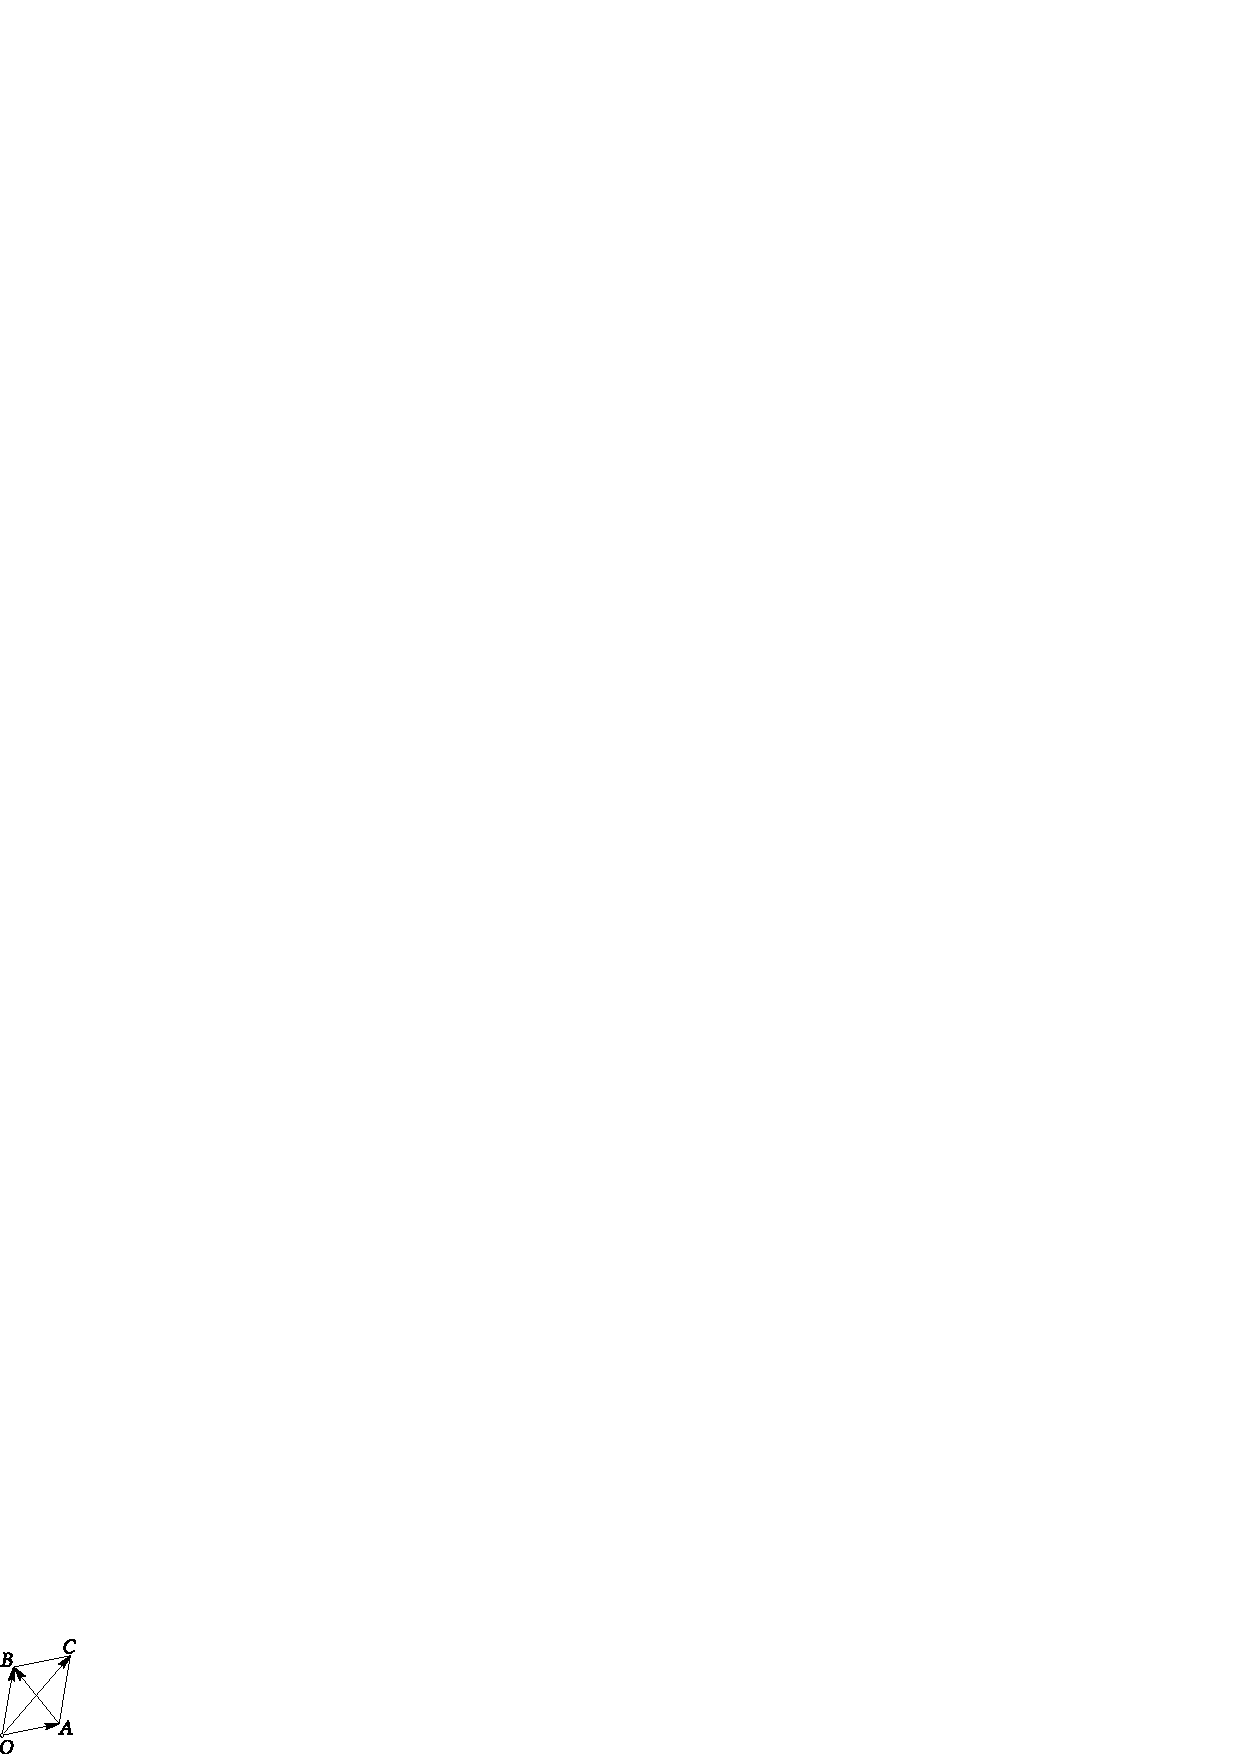
\includegraphics{05diagonals.pdf}}
Suppose you have a parallelogram one of whose vertices is the origin.
Label the vertices, starting at the origin and going around
counterclockwise, $O$, $A$, $C$ and $B$.  Let $\va=\tpv OA$, $\vb=\tpv
OB$, $\vc=\tpv OC$. One has
\[
  \tpv OC=\vc=\va+\vb,\quad\text{ and }\quad
  \tpv AB = \vb-\va.
\]
These vectors correspond to the diagonals $OC$ and $AB$ 
\begin{theorem}
  In a parallelogram $OACB$ the sum of the squares of the lengths of
  the two diagonals equals the sum of the squares of the lengths of
  all four sides.
\end{theorem}
\begin{proof}
The squared lengths of the diagonals are
\begin{align*}
  \|\tpv OC\|^2 = \|\va+\vb\|^2 &=\|\va\|^2+2\va\dpp\vb+\|\vb\|^2 \\
  \|\tpv AB\|^2 = \|\va-\vb\|^2 &=\|\va\|^2-2\va\dpp\vb+\|\vb\|^2
\end{align*}
Adding both these equations you get
\[
  \|\tpv OC\|^2 + \|\tpv AB\|^2 = 2\left(\|\va\|^2  +\|\vb\|^2 \right).
\]
The squared lengths of the sides are
\[
  \|\tpv OA\|^2=\|\va\|^2,\quad
  \|\tpv AB\|^2=\|\vb\|^2,\quad
  \|\tpv BC\|^2=\|\va\|^2,\quad
  \|\tpv OC\|^2=\|\vb\|^2.
\]
Together these also add up to $ 2\left(\|\va\|^2  +\|\vb\|^2 \right)$.
\end{proof}


\subsection{The dot product and the angle between two vectors} 
\label{sec:dot-prod-angle}

\begin{figure}[h]\label{fig:law-of-cosines} \centering
  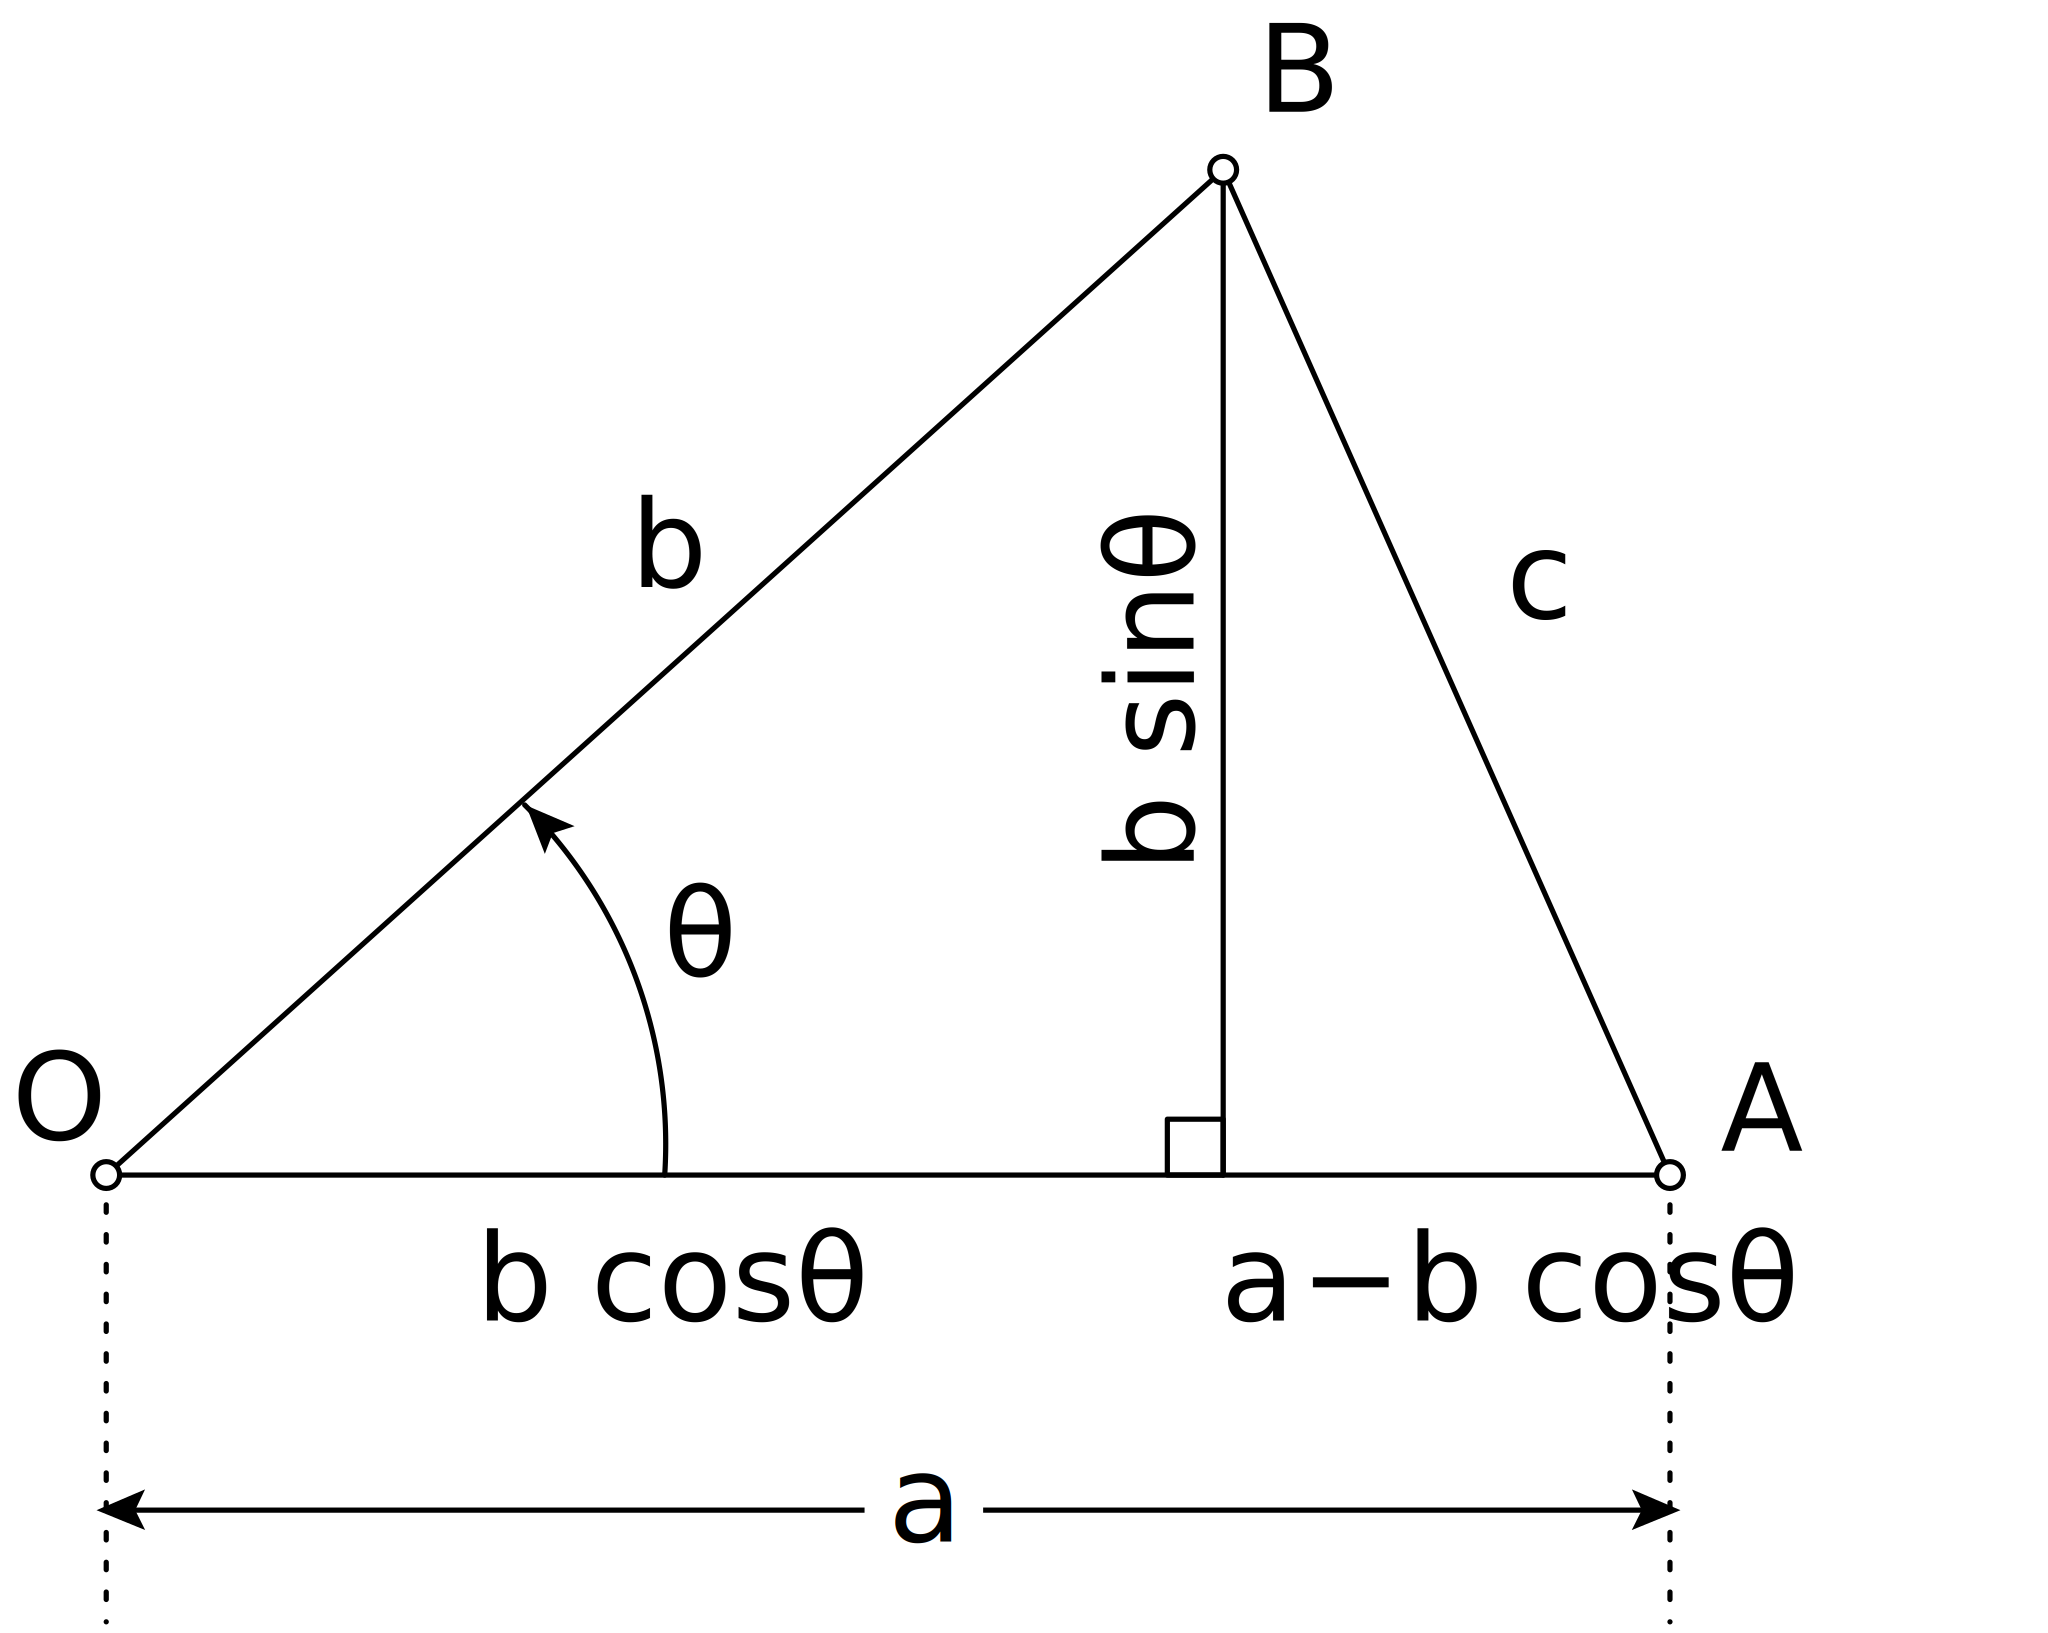
\includegraphics{05lawofcosines.pdf}
  \caption{Proof of the law of cosines}
\end{figure}
Here is the most important interpretation of the dot product:
\begin{theorem}
  If the angle between two vectors $\va$ and $\vb$ is $\theta$, then
  one has
  \[
    \va\dpp\vb = \|\va\| \, \|\vb\| \, \cos\theta.
  \]
\end{theorem}
An important special case is where the vectors $\va$ and $\vb$ are
perpendicular.  In that case $\theta=\frac\pi2$, so that $\cos \theta=0$ and the
dot product of $\va$ and $\vb$ vanishes.  Conversely, if both $\va$ and $\vb$
are non zero vectors whose dot product vanishes, then $\cos\theta$ must vanish,
and therefore $\theta=\frac\pi2$.  In short, \textit{two non-zero vectors are
perpendicular if and only if their dot product vanishes.}
\begin{proof}
We need \textit{the law of cosines} from high-school trigonometry.
Recall that for a triangle $OAB$ with angle $\theta$ at the point
$O$, and with sides $OA$ and $OB$ of lengths $a$ and $b$, the length
$c$ of the opposing side $AB$ is given by
\begin{equation}
  \label{eq:law-of-cosines}
  c^2 = a^2+b^2-2ab\cos\theta.
\end{equation}
In trigonometry this is proved by dropping a perpendicular line from
$B$ onto the side $OA$. The triangle $OAB$ gets divided into two
right triangles, one of which has $AB$ as hypotenuse. Pythagoras
then implies
\[
  c^2= \left(b\sin\theta\right)^2+\left(a-b\cos\theta\right)^2.
\]
After simplification you get (\ref{eq:law-of-cosines}).

To prove the theorem you let $O$ be the origin, and then observe
that the length of the side $AB$ is the length of the vector $\tpv
AB = \vb-\va$. Here $\va=\tpv OA$, $\vb=\tpv OB$, and hence
\[
  c^2=\|\vb-\va\|^2
  = (\vb-\va)\dpp (\vb-\va)
  =\|\vb\|^2+\|\va\|^2-2\va\dpp\vb.
\]
Compare this with (\ref{eq:law-of-cosines}), keeping in mind that
$a=\|\va\|$ and $b=\|\vb\|$: you are led to conclude that
$-2\va\dpp\vb = -2ab\cos\theta$, and thus $\va\dpp\vb =
\|\va\|\,\|\vb\|\cos\theta$.
\end{proof}



\subsection{Orthogonal projection of one vector onto another} 
\label{sec:orth-proj-vect}
The following construction comes up very often. Let $\va\neq\vvv0$ be
a given vector. Then for any other vector $\vx$ there is a number
\marginpar{\parbox{96pt}{\small\sffamily\centering\color{darkbluegreen}
\input{../figures/222/05orthogonal-decomposition.pdf_tex} 
Given $\vx$ and $\va$,\\
find $\vx^\perp$ and $\vx^\pll$. 
\rule[-8pt]{0pt}{1pt}
}}
$\lambda$ such that
\[
  \vx = \lambda \va + \vy
\]
where $\vy\perp\va$. In other words, you can write any vector $\vx$ as
the sum of one vector parallel to $\va$ and another vector orthogonal to
$\va$. The two vectors $\lambda\va$ and $\vy$ are called the
\emph{parallel} and \emph{orthogonal components} of the vector $\vx$
(with respect to $\va$), and sometimes the following notation is used
\[
  \vx^\pll= \lambda\va,\qquad \vx^\perp = \vy,
\]
so that
\[
  \vx=\vx^\pll+\vx^\perp.
\]
There are moderately simple formulas for $\vx^\pll$ and $\vx^\perp$,
but it is better to remember the following derivation of these
formulas.

Assume that the vectors $\va$ and $\vx$ are given. Then we look for a
number $\lambda$ such that $\vy = \vx-\lambda\va$ is perpendicular to
$\va$. Recall that $\va\perp (\vx-\lambda\va)$ if and only if 
\[
  \va\dpp (\vx-\lambda\va) = 0.
\]
Expand the dot product and you get this equation for $\lambda$
\[
  \va\dpp\vx - \lambda\va\dpp\va = 0,
\]
whence
\begin{equation}
  \label{eq:parallel-component}
  \lambda = \frac{\va\dpp\vx}{\va\dpp\va}= \frac{\va\dpp\vx}{\nm\va^2}
\end{equation}
To compute the parallel and orthogonal components of $\vx$
w.r.t.~$\va$ you first compute $\lambda$ according to
(\ref{eq:parallel-component}), which tells you that the parallel
component is given by
\[
  \vx^\pll=\lambda\va = \frac{\va\dpp\vx}{\va\dpp\va}\;\va.
\]
The orthogonal component is then ``the rest,'' i.e.~by definition
$\vx^\perp=\vx-\vx^\pll$, so
\[
  \vx^\perp = \vx-\vx^\pll= \vx-\frac{\va\dpp\vx}{\va\dpp\va}\;\va.
\]

\subsection{Defining equations of lines} 
\label{sec:equat-lines-plan}

In \S~\ref{sec:param-equat-lines} we saw how to generate points on a
line given two points on that line by means of a ``parametrization.''
I.e.~given points $A$ and $B$ on the line $\ell$ the point whose
position vector is $\vx=\va+t (\vb-\va)$ will be on $\ell$ for any
value of the ``parameter'' $t$.

In this section we will use the dot-product to give a different
description of lines in the plane (and planes in three dimensional
space.)  We will derive an equation for a line. Rather than generating
points on the line $\ell$ this equation tells us if any given point
$X$ in the plane is on the line or not.

Here is the derivation of the equation of a line in the plane. To
produce the equation you need two ingredients:

\textbf{1. } One particular point on the line (let's call this point
$A$, and write $\va$ for its position vector),

\textbf{2. } a \emph{normal vector} $\vn$ for the line, i.e.~a nonzero
vector which is perpendicular to the line.

\noindent Now let $X$ be any point in the plane, and consider the line
segment $AX$.

\begin{itemize}
\item Clearly, $X$ will be on the line if and only if $AX$ is parallel
  to $\ell$ \footnote{ From plane Euclidean geometry: parallel lines
  either don't intersect or they coincide.}

\item Since $\ell$ is perpendicular to $\vn$, the segment $AX$ and the
  line $\ell$ will be parallel if and only if $AX\perp\vn$.
\item $AX\perp\vn$ holds if and only if $\tpv AX\dpp\vn=0$. 
\end{itemize}
So in the end we see that $X$ lies on the line $\ell$ if and only if
the following vector equation is satisfied:
\begin{equation}
  \label{eq:line-defined-by-dotp}
  \tpv AX\dpp\vn=0\quad\text{or}\quad \left(\vx-\va\right)\dpp\vn=0
\end{equation}
This equation is called a \emph{defining equation for the line $\ell$. }

Any given line has many defining equations. Just by changing the
length of the normal you get a different equation, which still
describes the same line.

\begin{figure}[h]
  \centering \input{../figures/222/05equation4line.pdf_tex}

  \caption{If $\vn$ is a normal vector to the line $\ell$, and if $A$ is
  any point on $\ell$, then there is a simple test which tells you if a
  point $X$ is on $\ell$ or not: $X$ is on $\ell$ if and only if $\tpv
  AX\perp\vn$, i.e.\ iff $\tpv AX \dpp \vn=0$.}
  \label{fig:05equation4line}
\end{figure}

\subsection{Line through one point and perpendicular to another line} 
\textit{Find a defining equation for the line $\ell$ which goes
through $A (1,1)$ and is perpendicular to the line segment $AB$ where
$B$ is the point $(3,-1)$.}

\begin{figure}
  \input{../figures/222/05line-perp2AB.pdf_tex}
\end{figure}

\textit{Solution. } We already know a point on the line, namely $A$,
but we still need a normal vector. The line is required to be
perpendicular to $AB$, so $\vn=\tpv AB$ is a normal vector:
\[
  \vn =\tpv AB = \vek 3-1 \\(-1)-1 \tor = \vek 2 \\-2  \tor
\]
Of course any multiple of $\vn$ is also a normal vector, for instance
\[
  \vm = \tfrac12\vn = \vek 1\\ -1\tor
\]
is a normal vector.

With $\va=\tvek 1 \\1\ttor$ we then get the following equation for $\ell$
\[
  \vn\dpp (\vx-\va)= \vek 2 \\-2  \tor\dpp\vek x_1-1 \\x_2-1\tor =
  2x_1-2x_2=0.
\]
If you choose the normal $\vm$ instead, you get
\[
  \vm\dpp (\vx-\va)= \vek 1 \\-1  \tor\dpp\vek x_1-1 \\x_2-1\tor =
  x_1-x_2=0.
\]
Both equations $2x_1-2x_2=0 $  and $x_1-x_2=0 $ are equivalent and they both give
defining equations for the line $\ell$.

\subsection{Distance to a line} 
\label{sec:distance-line}

Let $\ell$ be a line in the plane and assume a point $A$ on the line
as well as a vector $\vn$ perpendicular to $\ell$ are known. Using the
dot product one can easily compute the distance from the line to any
other given point $P$ in the plane. Here is how:

Draw the line $m$ through $A$ perpendicular to $\ell$, and drop a
perpendicular line from $P$ onto $m$. let $Q$ be the projection of $P$
onto $m$. The distance from $P$ to $\ell$ is then equal to the length
of the line segment $AQ$. Since $AQP$ is a right triangle one has
\[
  AQ = AP\cos\theta.
\]
Here $\theta$ is the angle between the normal $\vn$ and the vector
$\tpv AP$. One also has
\[
  \vn\dpp (\vp-\va) = \vn\dpp \tpv AP= \nm{\tpv AP}\;\nm \vn \cos \theta
  =AP\nm\vn\cos\theta.
\]
Hence we get
\[
  \mathrm{dist} (P,\ell) = \frac{\vn\dpp (\vp-\va)}{\nm\vn}.
\]
\begin{figure}[h]
  \input{../figures/222/05distance-to-line.pdf_tex}
  \caption{The distance from a point $P$ to a line $\ell$.  }
  \label{fig:05distance-to-line}
\end{figure}
This argument from a drawing contains a hidden assumption, namely that the point
$P$ lies on the side of the line $\ell$ pointed to by the vector $\vn$. If this
is not the case, so that $\vn$ and $\tpv AP$ point to opposite sides of $\ell$,
then the angle between them exceeds $90^\circ$, i.e.~$\theta>\pi/2$. In this
case $\cos\theta<0$, and one has $AQ=-AP\cos \theta$. The distance formula
therefore has to be modified to
\[
  \mathrm{dist} (P,\ell) =- \frac{\vn\dpp (\vp-\va)}{\nm\vn}.
\]
We do not need to know in advance which formula to use.  If we compute $\vn \dpp
(\vp-\va)$ and find that it is negative then we know that the normal vector
and the point are on opposite sides of the line $\ell$.  In either case the
distance is given by
\[
  \mathrm{dist} (P,\ell) = \left| \frac{\vn\dpp (\vp-\va)}{\nm\vn}\right|.
\]

\subsection{Defining equation of a plane} 
\label{sec:defin-equat-plane}
Just as we have seen how we can form the defining equation for a line
in the plane from just one point on the line and one normal vector to
the line, we can also form the defining equation for a plane in
space, again knowing only one point on the plane, and a vector
perpendicular to it.
\begin{figure}[b]
  \centering
  \input{../figures/222/05equation4plane.pdf_tex}
  \caption{A point $P$ lies on the plane if the vector $\tpv AP$ is
  perpendicular to $\vn$.}
\end{figure}
If $A$ is a point on some plane $\cP$ and $\vn$ is a vector
perpendicular to $\cP$, then any other point $X$ lies on $\cP$ if and
only if $\tpv AX\perp\vn$. In other words, in terms of the position
vectors $\va$ and $\vx$ of $A$ and $X$,
\[
  \text{the point $X$ is on $\cP$} \iff \vn\dpp (\vx-\va)=0.
\]
Arguing just as in \S~\ref{sec:distance-line} you find that the
distance of a point $X$ in space to the plane $\cP$ is
\begin{equation}\label{eq:dist-point2plane}
  \mathrm{dist} (X,\cP) = \pm\frac{\vn\dpp (\vx-\va)}{\nm\vn}.
\end{equation}
Here the sign is ``$+$'' if $X$ and the normal $\vn$ are on the same
side of the plane $\cP$; otherwise the sign is ``$-$''.
\subsection{Example}  \label{ex:defining-eqn-plane} 
Find the defining equation for the plane $\cP$ through the
point $A (1,0,2)$ which is perpendicular to the vector $\tvek
1\\2\\1\ttor$.

\textit{Solution: } We know a point ($A$) and a normal vector
$\vn=\tvek 1 \\ 2\\ 1\ttor$ for $\cP$. Then any point $X$ with
coordinates $(x_1,x_2,x_3)$, or, with position vector $\vx=\tvek x_1
\\x_2\\x_3\ttor$, will lie on the plane $\cP$ if and only if
\begin{align*}
  \vn\dpp (\vx-\va)=0&\iff 
  \vek 1 \\ 2\\ 1\tor \dpp
  \left\{\vek x_1\\x_2\\x_3\tor-\vek1\\0\\2\tor
  \right\}=0 \\
  &\iff
  \vek 1 \\ 2\\ 1\tor \dpp\vek x_1-1 \\ x_2 \\ x_3-2\tor=0 \\
  & \iff
  1\cdot(x_1-1)+ 2\cdot(x_2) + 1\cdot ( x_3-2) =0\\
  &\iff x_1+2x_2+x_3 - 3=0.
\end{align*}
\begin{figure}[h]
  \centering
  \input{../figures/222/05ex-plane.pdf_tex}
  \label{fig:example-of-plane}
\end{figure}

\subsection{Example continued} 
Let $\cP$ be the plane from the previous example. Which of
the points $P(0,0,1)$, $Q (0,0,2)$, $R (-1,2,0)$ and $S (-1, 0,
5)$ lie on $\cP$? Compute the distances from the points $P,Q,R,S$
to the plane $\cP$. Separate the points which do not lie on $\cP$
into two group of points which lie on the same side of $\cP$. 

\textit{Solution: } We apply (\ref{eq:dist-point2plane}) to the
position vectors $\vp,\vq,\vr,\vs$ of the points $P,Q,R,S$. For each
calculation we need  
\[
  \nm\vn = \sqrt{1^2+2^2+1^2}=\surd6.
\]
The third component of the given normal $\vn=\tvek 1\\2\\1\ttor$ is
positive, so $\vn$ points ``upwards.'' Therefore, if a point lies on
the side of $\cP$ pointed to by $\vn$, we shall say that the point
lies \textit{above the plane.} 
\begin{description}
\item[$P$] $\vp=\tvek 0\\0\\1\ttor$, $\vp-\va=\tvek -1 \\ 0
  \\-1\ttor$, $ \vn\dpp (\vp-\va) = 1\cdot (-1)+2\cdot (0)+1\cdot
  (-1) = -2 $
  \[
    \frac{\vn\dpp (\vp-\va)}{\nm\vn} = -\frac2{\surd6}=-\frac13\surd6.
  \]
  This quantity is negative, so $P$ lies below $\cP$. Its distance
  to $\cP$ is $\frac13\surd6$.
  \goodbreak

\item[$Q$] $\vq=\tvek 0\\0\\2\ttor$, $\vp-\va=\tvek -1 \\ 0
  \\0\ttor$, $ \vn\dpp (\vp-\va) = 1\cdot (-1)+2\cdot (0)+1\cdot
  (0) = -1 $
  \[
    \frac{\vn\dpp (\vp-\va)}{\nm\vn} = -\frac1{\surd6}=-\frac16\surd6.
  \]
  This quantity is negative, so $Q$ also lies below $\cP$. Its
  distance to $\cP$ is $\frac16\surd6$.

\item[$R$] $\vr=\tvek -1\\2\\0\ttor$, $\vp-\va=\tvek -2 \\ 2
  \\ -2\ttor$, $ \vn\dpp (\vp-\va) = 1\cdot (-2)+2\cdot (2)+1\cdot
  (-2) = 0 $
  \[
    \frac{\vn\dpp (\vp-\va)}{\nm\vn} = 0.
  \]
  Thus $R$ lies on the plane $\cP$, and its distance to $\cP$ is of
  course $0$.

\item[$S$] $\vs=\tvek -1\\0\\5\ttor$, $\vp-\va=\tvek -2 \\ 0
  \\3\ttor$, $ \vn\dpp (\vp-\va) = 1\cdot (-1)+2\cdot (0)+1\cdot
  (3) = 2 $
  \[
    \frac{\vn\dpp (\vp-\va)}{\nm\vn} = \frac2{\surd6}=\frac13\surd6.
  \]
  This quantity is positive, so $S$ lies above $\cP$. Its distance
  to $\cP$ is $\frac13\surd6$.
\end{description}
We have found that $P$ and $Q$ lie below the plane, $R$ lies on the plane,
and $S$ is above the plane.

\subsection{Where does the line through the points $B (2,0,0)$ and $C 
(0,1,2)$ intersect the plane $\cP$ from example
\ref{ex:defining-eqn-plane}?}

\textit{Solution: } Let $\ell$ be the line through $B$ and $C$. We
set up the parametric equation for $\ell$. According to
\S\ref{sec:param-equat-lines}, (\ref{eq:line-parametric}) every
point $X$ on $\ell$ has position vector $\vx$ given by
\begin{equation}
  \label{eq:line-intersect-plane1}
  \vx = \vb+t (\vc-\vb)
  = \vek2\\0\\0\tor + t\vek 0-2\\1-0\\2-0\tor 
  = \vek 2-2t \\ t \\ 2t \tor
\end{equation}
for some value of $t$.

The point $X$ whose position vector $\vx$ is given above lies on the
plane $\cP$ if $\vx$ satisfies the defining equation of the plane.
In example \ref{ex:defining-eqn-plane} we found this defining
equation. It was
\begin{equation}
  \label{eq:line-intersect-plane2}
  \vn\dpp (\vx-\va) =0, \text{~i.e.~} x_1+2x_2+x_3 - 3=0.
\end{equation}
So to find the point of intersection of $\ell$ and $\cP$ you
substitute the parametrization (\ref{eq:line-intersect-plane1}) in
the defining equation (\ref{eq:line-intersect-plane2}):
\[
  0=x_1+2x_2+x_3 - 3= (2-2t)+2 (t)+ (2t)-3 = 
  2t-1.
\]
This implies $t=\frac12$, and thus the intersection point has
position vector
\[
  \vx = \vb+\tfrac12 (\vc-\vb) = \vek 2-2t \\ t \\ 2t \tor
  =\vek 1 \\ \tfrac12 \\ 1\tor,
\]
i.e.~$\ell$ and $\cP$ intersect at $X (1,\frac12,1)$.


\section{Cross Product}\label{sec:cross-product} 

\subsection{Algebraic definition of the cross product} 
\label{sec:algebr-defin-cross}
Here is the definition of the cross-product of two vectors. The
definition looks a bit strange and arbitrary at first sight -- it
really makes you wonder who thought of this.  We will just put up with
that for now and explore the properties of the cross product. Later on
we will see a geometric interpretation of the cross product which will
show that this particular definition is really useful. We will also
find a few tricks that will help you reproduce the formula without
memorizing it.
\begin{definition}
  The ``outer product'' or ``cross product'' of two vectors is given
  by
  \[
    \vek a_1\\a_2\\a_3\tor \cp \vek b_1\\b_2\\b_3\tor = 
    \vek a_2b_3-a_3b_2 \\ a_3b_1-a_1b_3 \\ a_1b_2-a_2b_1 \tor 
  \]
\end{definition}
Note that the cross-product of two vectors is again a vector! 

\subsection{Example} 
If you set $\vb=\va$ in the definition you find the following
important fact: \textit{The cross product of any vector with itself
is the zero vector:}
\[
  \va\cp\va = \vvv0 \quad \text{for \emph{any} vector $\va$.}
\]

\subsection{Example} 
Let $\va=\tvek 1\\2\\3\ttor$, $\vb=\tvek -2\\1 \\0\ttor$ and compute
the cross product of these vectors.

\textit{Solution: }
\[
  \va\cp\vb = \vek 1\\2\\3\tor \cp\vek -2\\1 \\0\tor
  =\left(
  \begin{aligned}
    2\cdot0&-3\cdot1 \\ 3\cdot (-2)&-1\cdot0 \\ 1\cdot1&-2\cdot (-2)
  \end{aligned}
  \right)
  =\vek -3 \\ -6 \\ 5
  \tor
\]
\subsection{Algebraic properties of the cross product} 
\label{sec:algebr-prop-cross}
Unlike the dot product, the cross product of two vectors behaves much
less like ordinary multiplication. To begin with, the product is
\emph{not commutative} -- instead one has
\begin{equation}
  \va\cp\vb = -\vb\cp\va \quad \text{for \emph{all} vectors $\va$ and $\vb$}.
\end{equation}
This property is sometimes called ``anti-commutative.''

\marginpar{\footnotesize\sffamily
$\vi\cp  (\vi\cp\vj)=  -\vj$,\\ and \\
$(\vi\cp \vi)\cp\vj = \vvv0$,\\
so\\ $\vi\cp  (\vi\cp\vj)$\\
\null\quad$\not= (\vi\cp \vi)\cp\vj$ \\Conclusion:\\
``$\cp$'' is not associative}

Since the crossproduct of two vectors is again a vector you can
compute the cross product of three vectors $\va,\vb,\vc$. You now have
a choice: do you first multiply $\va$ and $\vb$, or $\vb$ and $\vc$,
or $\va$ and $\vc$? With numbers it makes no difference (e.g.~$2\times
(3\times5)=2\times15=30$ and $(2\times3)\times5=6\times5=$ also $30$)
but with the cross product of vectors it does matter: the cross
product is \emph{not associative,} i.e.  
\[
  \va \cp (\vb\cp\vc) \pmb{\neq} (\va\cp\vb)\cp\vc \quad
  \text{for \emph{most}  vectors }\va,\vb,\vc.
\]
The \emph{distributive law} does hold, i.e.
\[
  \va\cp (\vb+\vc) = \va\cp\vb + \va\cp\vc,\quad \text{and}\quad
  (\vb+\vc)\cp\va = \vb\cp\va+\vc\cp\va
\]
is true for all vectors $\va,\vb,\vc$.

Also, an associative law, where one of the factors is a number and the
other two are vectors, does hold. I.e.
\[
  t (\va\cp\vb ) = (t\va)\cp\vb = \va\cp (t\vb)
\]
holds for all vectors $\va,\vb$ and any number $t$.  We were already
using these properties when we multiplied $(a_1\vi+a_2\vj+a_3\vk)\cp
(b_1\vi+b_2\vj+b_3\vk)$ in the previous section.

Finally, the cross product is only defined for space vectors, not for
plane vectors.

\subsection{Ways to compute the cross product} 
In terms of the standard basis vectors you can check the
\textit{multiplication table}.  An easy way to remember the
multiplication table is to put the vectors $\vi,\vj,\vk$ clockwise in
a circle. Given two of the
three vectors their product is either plus or minus the remaining
vector. To determine the sign you step from the first vector to the
second, to the third: if this makes you go clockwise you have a plus
sign, if you have to go counterclockwise, you get a minus.
\marginpar{\centering
\parbox[b]{102pt}
{\centering
\(\displaystyle
\begin{array}[c]{c|ccc}
  \cp & \vi   &   \vj   & \vk \\ \hline 
  \rule{0pt}{14pt}\vi &\vvv0  &   \vk   & -\vj \\
  \vj &  -\vk &  \vvv0  & \vi \\
  \vk &  \vj  &  -\vi   &  \vvv 0
\end{array}
\)
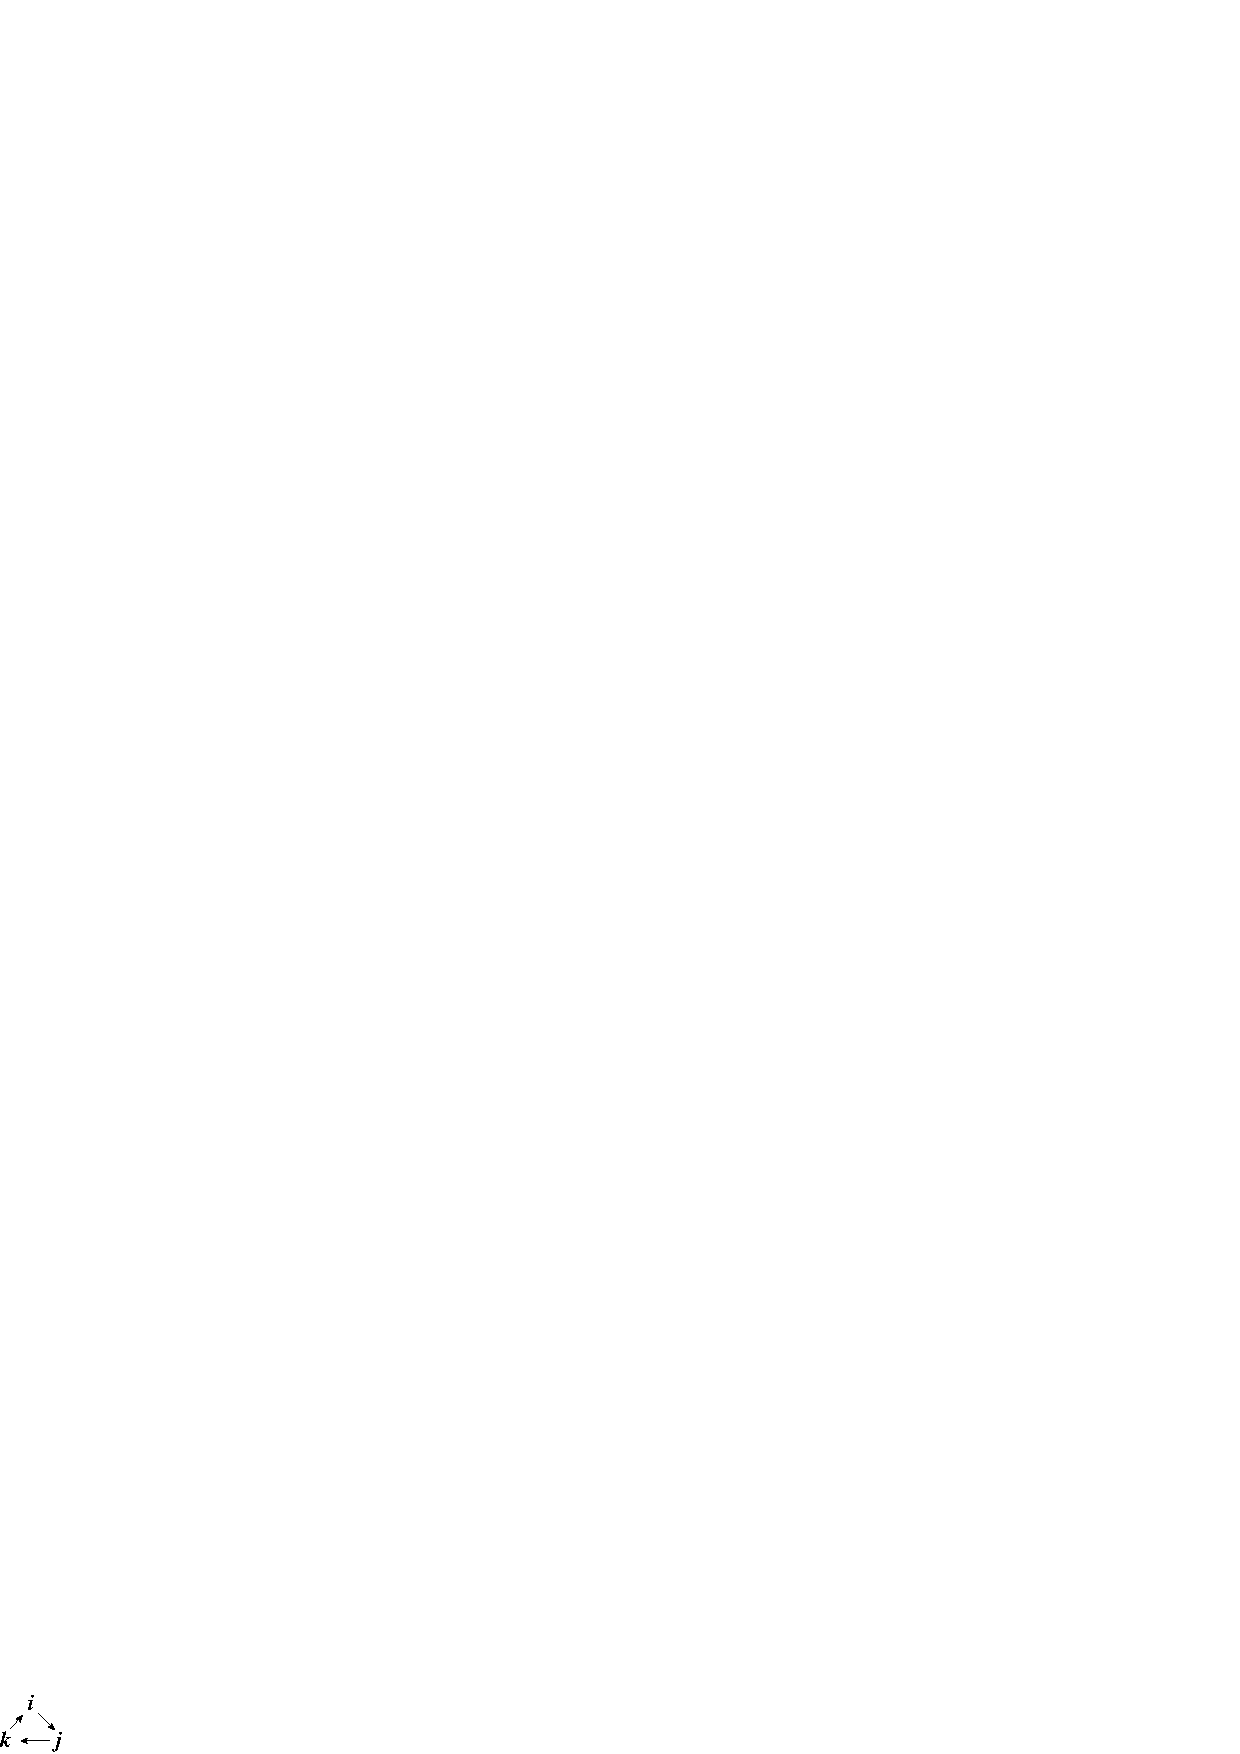
\includegraphics{05ijk-cyclic.pdf}
}}

The products of $\vi,\vj$ and $\vk$ are all you need to know to
compute the cross product. Given two vectors $\va$ and $\vb$ write
them as $\va=a_1\vi+a_2\vj+a_3\vk$ and $\vb=b_1\vi+b_2\vj+b_3\vk$, and
multiply as follows
\begin{align*}
  \va\cp\vb
  =& (a_1\vi+a_2\vj+a_3\vk)\cp (b_1\vi+b_2\vj+b_3\vk) \\
  =&
  \begin{array}[t]{r}
    a_1\vi\cp (b_1\vi+b_2\vj+b_3\vk) \\
    +a_2\vj\cp (b_1\vi+b_2\vj+b_3\vk) \\
    +a_3\vk\cp (b_1\vi+b_2\vj+b_3\vk) 
  \end{array}\\
  =& 
  \begin{array}[t]{rccccc}
    a_1b_1\vi\cp\vi & + &a_1b_2\vi\cp\vj & + & a_1b_3\vi\cp\vk & +\\
    a_2b_1\vj\cp\vi & + &a_2b_2\vj\cp\vj & + & a_2b_3\vj\cp\vk & +\\
    a_3b_1\vk\cp\vi & + &a_3b_2\vk\cp\vj & + & a_3b_3\vk\cp\vk &
  \end{array} \\
  =&
  \begin{array}[t]{cccccc}
    a_1b_1\vvv0 & + &a_1b_2\vk & - & a_1b_3\vj & \\
    -a_2b_1\vk & + &a_2b_2\vvv0 & + & a_2b_3\vi & +\\
    a_3b_1\vj & - &a_3b_2\vi & + & a_3b_3\vvv0 &
  \end{array} \\
  =&( a_2b_3- a_3b_2)\vi + ( a_3b_1-a_1b_3)\vj + (a_1b_2 -a_2b_1)\vk
\end{align*}
This is a useful way of remembering how to compute the cross product,
particularly when many of the components $a_i$ and $b_j$ are zero.

\subsection{Example} 
Compute $\vk\cp (p\vi+q\vj+r\vk)$:
\[
  \vk\cp (p\vi+q\vj+r\vk)  = p (\vk\cp\vi)+q (\vk\cp\vj)+r (\vk\cp\vk)
  =-q\vi+p\vj.
\]

There is another way of remembering how to find $\va\cp\vb$. It
involves the ``triple product'' and determinants. See
\S~\ref{sec:triple-product}.


\subsection{The triple product and determinants} 
\label{sec:triple-product}
\begin{definition}
  The triple product of three given vectors $\va,\vb$, and $\vc$ is
  defined to be 
  \[
    \va\dpp (\vb\cp\vc).
  \]
\end{definition}
In terms of the components of $\va,\vb$, and $\vc$ one has

\begin{align*}
  \va\dpp (\vb\cp\vc) &= 
  \vek a_1\\a_2\\a_3\tor \dpp
  \vek b_2c_3-b_3c_2 \\ b_3c_1-b_1c_3 \\ b_1c_2 - b_2 c_1 \tor \\
  &=
  a_1b_2c_3 - a_1b_3c_2 + a_2b_3c_1 - a_2b_1c_3 + a_3b_1c_2 - a_3b_2c_1.
\end{align*}
This quantity is called a \emph{determinant,} and is written as
follows
\begin{equation}
  \label{eq:determinant-def}
  \left|
  \begin{matrix}
    a_1 & b_1 & c_1 \\a_2 & b_2 & c_2 \\ a_3 & b_3 & c_3
  \end{matrix}
  \right| 
  = a_1b_2c_3 - a_1b_3c_2 + a_2b_3c_1 - a_2b_1c_3 + a_3b_1c_2 - a_3b_2c_1 
\end{equation}

\centerline{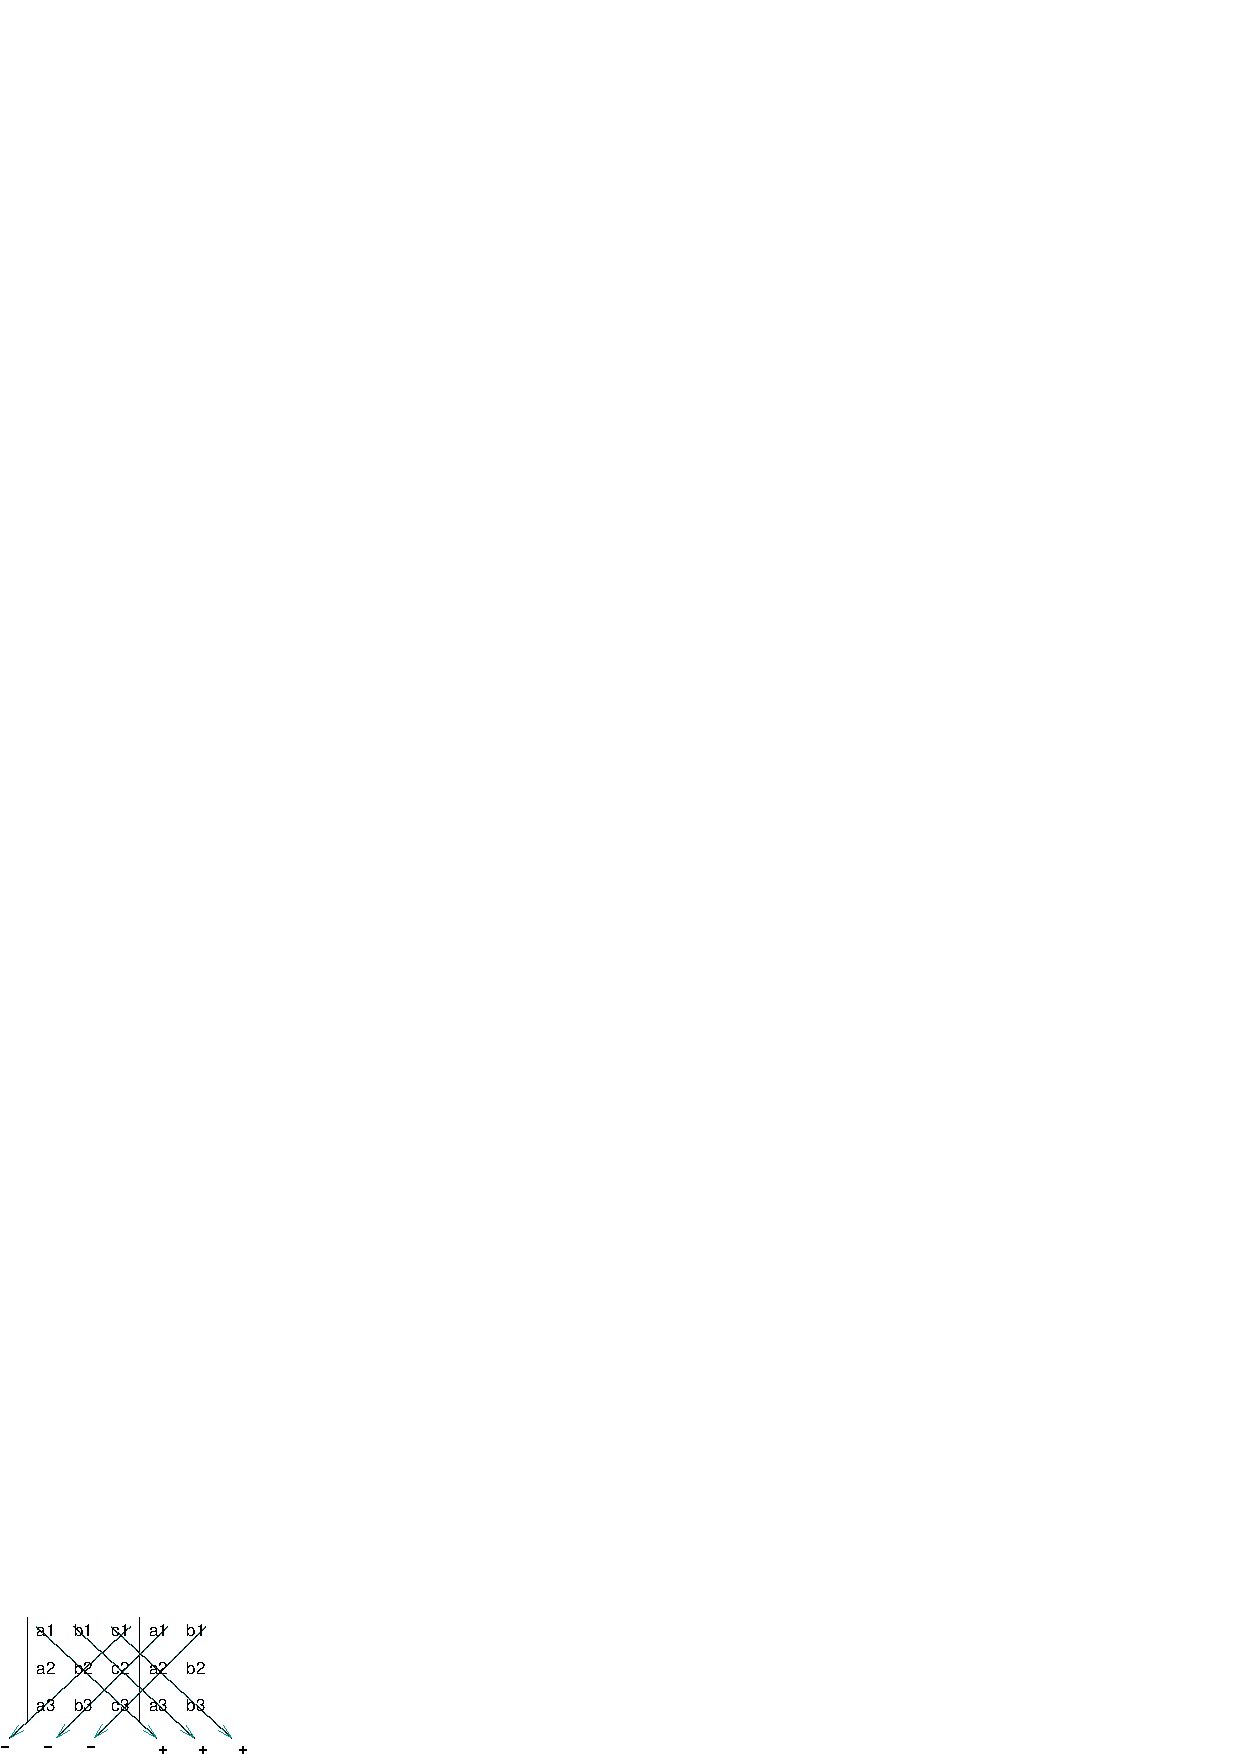
\includegraphics{05determinant-shortcut.pdf}}
There's a useful shortcut for computing such a determinant: after
writing the determinant, append a fourth and a fifth column which
are just copies of the first two columns of the determinant. The
determinant then is the sum of six products, one for each dotted
line in the drawing. Each term has a sign: if the factors are read
from top-left to bottom-right, the term is positive, if they are
read from top-right to bottom left the term is negative.
This shortcut is also very useful for computing the crossproduct. To
compute the cross product of two given vectors $\va$ and $\vb$ you
arrange their components in the following determinant
\begin{equation}\label{eq:cross-prod-shortcut}
  \va\cp\vb =   \left|
  \begin{matrix}
    \vi &  a_1 & b_1 \\ \vj & a_2 & b_2  \\ \vk & a_3 & b_3
  \end{matrix}
  \right| 
  = ( a_2b_3- a_3b_2)\vi + ( a_3b_1-a_1b_3)\vj + (a_1b_2 -a_2b_1)\vk.
\end{equation}
This is not a normal determinant since some of its entries are
vectors, but if you ignore that odd circumstance and simply compute
the determinant according to the definition
(\ref{eq:determinant-def}), you get (\ref{eq:cross-prod-shortcut}).


An important property of the triple product is that it is much more
symmetric in the factors $\va,\vb,\vc$ than the notation $\va\dpp
(\vb\cp\vc)$ suggests.
\begin{theorem}
  For any triple of vectors $\va,\vb,\vc$ one has
  \[
    \va\dpp (\vb\cp\vc) = \vb\dpp (\vc\cp\va) = \vc\dpp (\va\cp\vb),
  \]
  and 
  \[
    \va\dpp (\vb\cp\vc) = -\vb\dpp (\va\cp\vc) = -\vc\dpp (\vb\cp\va).
  \]
\end{theorem}
In other words, if you exchange two factors in the product $\va\dpp
(\vb\cp\vc)$ it changes its sign. If you ``rotate the factors,''
i.e.~if you replace $\va$ by $\vb$, $\vb$ by $\vc$ and $\vc$ by $\va$,
the product doesn't change at all.


\subsection{Geometric description of the cross product} 
\label{sec:geom-descr-cross}
\begin{theorem}
  \[
    \va\cp\vb \perp \va,\vb
  \]
\end{theorem}
\begin{proof}
We use the triple product:
\[
  \va\dpp (\va\cp\vb) = \vb\dpp (\va\cp\va) = 0
\]
since $\va\cp\va=\vvv0$ for any vector $\va$. It follows that
$\va\cp\vb$ is perpendicular to $\va$.

\marginpar{  \centering
\input{../figures/222/05crossprod.pdf_tex}}
Similarly, $\vb\dpp (\va\cp\vb) = \va\dpp (\vb\cp\vb) = 0$ shows
that $\va\dpp\vb$ is perpendicular to $\vb$.
\end{proof}

\begin{theorem}
  \[
    \|\va\cp\vb \| = \|\va\|\,\|\vb\|\,\sin\theta
  \]
\end{theorem}
\begin{proof}
Bruce\footnote{It's actually called \emph{Lagrange's identity}.  Yes, the same
Lagrange who found the formula for the remainder term in Taylor's
formula.} just slipped us a piece of paper with the following
formula on it:
\begin{equation}
  \label{eq:Lagrange-identity}
  \|\va\cp\vb\|^2 +  (\va\dpp\vb)^2 = \|\va\|^2\|\vb\|^2.
\end{equation}
After setting $\va=\tvek a_1\\a_2\\a_3\ttor$ and $\vb=\tvek b_1\\
b_2\\b_3\ttor$ and diligently computing both sides we find that this
formula actually holds for any pair of vectors $\va,\vb$!  The
(long) computation which implies this identity will be presented in
class (maybe).

If we assume that Lagrange's identity holds then we get
\[
  \|\va\cp\vb\|^2 =  \|\va\|^2\|\vb\|^2 -  (\va\dpp\vb)^2
  =  \|\va\|^2\|\vb\|^2 - \|\va\|^2\|\vb\|^2 \cos^2\theta
  =  \|\va\|^2\|\vb\|^2 \sin^2\theta
\]
since $1-\cos^2\theta=\sin^2\theta$. The theorem is proved.
\end{proof}

These two theorems \textit{almost} allow you to construct the cross
product of two vectors geometrically. If $\va$ and $\vb$ are two
vectors, then their cross product satisfies the following description:
\begin{enumerate}
\item If $\va$ and $\vb$ are parallel, then the angle $\theta$ between
  them vanishes, and so their cross product is the zero vector. Assume
  from here on that $\va$ and $\vb$ are not parallel.
\item $\va\cp\vb$ is perpendicular to both $\va$ and $\vb$. In other
  words, since $\va$ and $\vb$ are not parallel, they determine a
  plane, and their cross product is a vector perpendicular to this
  plane.
\item the length of the cross product $\va\cp\vb$ is
  $\nm\va\,\nm\vb\,\sin\theta$.
\end{enumerate}

There are only two vectors that satisfy conditions 2 and 3: to
determine which one of these is the cross product you must apply the
\emph{Right Hand Rule} (screwdriver rule, corkscrew rule, etc.) for
$\va,\vb,\va\cp\vb$: if you turn a screw whose axis is perpendicular
to $\va$ and $\vb$ in the direction from $\va$ to $\vb$, the screw
moves in the direction of $\va\cp\vb$.
\begin{figure}[t]\centering
  \input{../figures/222/05crossprod-corkscrew.pdf_tex}
  \caption{The right hand rule for the cross product.}
\end{figure}

Alternatively, without seriously injuring yourself, you should be able
to make a fist with your \emph{right} hand, and then stick out your
thumb, index and middle fingers so that your thumb is $\va$, your
index finger is $\vb$ and your middle finger is $\va\cp\vb$.  If you do this
with your left hand you will get $-\va\cp\vb$ instead of $\va\cp\vb$.


\section{A few applications of the cross product} 
\label{sec:volumes}


\subsection{Area of a parallelogram} 
\label{sec:area-parallelogram}

Let $ABCD$ be a parallelogram. Its area is given by ``height times
base,'' a formula which should be familiar from high school geometry.

\begin{figure}[h]
  \centering
  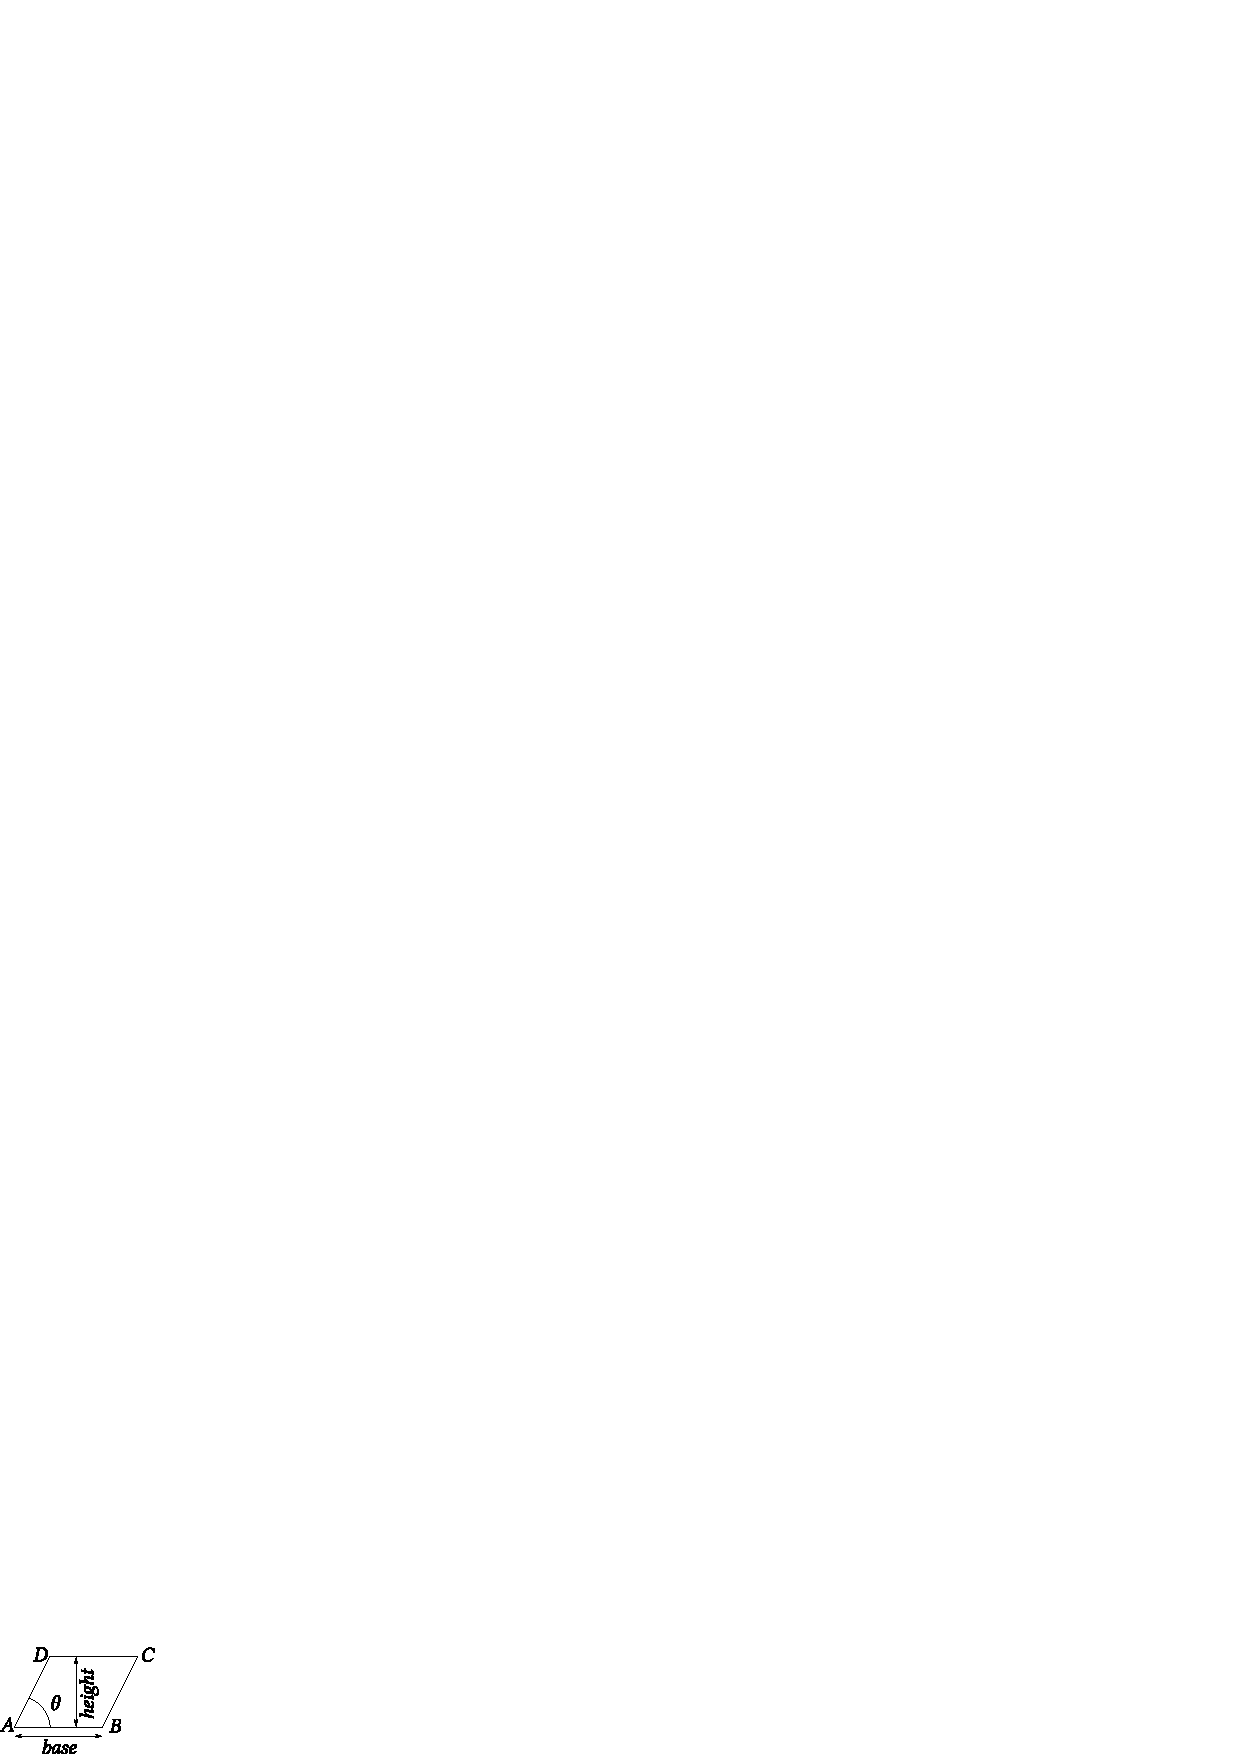
\includegraphics{05area-parallelogram.pdf}
  \caption{The area of a parallelogram}
\end{figure}
If the angle between the sides $AB$ and $AD$ is $\theta$, then the
height of the parallelogram is $\nm{\tpv AD}\sin\theta$, so that the
area of $ABCD$ is
\begin{equation}
  \label{eq:area-parallelogram}
  \text{area of }ABCD = \nm{\tpv AB}\,\nm{\tpv AD}\sin\theta
  = \nm{\tpv AB\cp\tpv AD}.
\end{equation}
The area of the triangle $ABD$ is of course half as much,
\[
  \text{area of triangle }ABD = \tfrac12 \nm{\tpv AB\cp\tpv AD}.
\]


These formulae are valid even when the points $A,B,C$, and $D$ are
points in space. Of course they must lie in one plane for otherwise
$ABCD$ couldn't be a parallelogram.
\subsection{Example} 
Let the points $A (1,0,2)$, $B (2,0,0)$, $C (3,1,-1)$ and $D
(2,1,1)$ be given.

\textit{Show that $ABCD$ is a parallelogram, and compute its area.}

\textit{Solution: } $ABCD$ will be a parallelogram if and only if
$\tpv AC=\tpv AB + \tpv AD$. In terms of the position vectors
$\va$,$\vb$, $\vc$ and $\vd$ of $A,B,C,D$ this boils down to
\[
  \vc-\va= (\vb-\va)+(\vd-\va),\quad\text{i.e. }\quad
  \va+\vc = \vb+\vd.
\]
For our points we get 
\[
  \va+\vc = \vek1\\0\\2\tor + \vek3\\1\\-1\tor = 
  \vek 4\\1\\1\tor,\qquad
  \vb+\vd = \vek 2\\0\\0\tor+\vek 2\\1\\1\tor = \vek 4\\1\\1\tor.
\]
So $ABCD$ is indeed a parallelogram. Its area is the length of
\[
  \tpv AB\cp\tpv AD = \vek 2-1\\0\\0-2\tor \cp \vek 2-1\\1-0\\1-2\tor
  =\vek 1\\0\\-2\tor \cp \vek 1\\-1\\-1\tor
  =\vek -2 \\-1\\-1\tor.
\]
So the area of $ABCD$ is $\sqrt{(-2)^2+ (-1)^2+ (-1)^2}=\sqrt6$.

\subsection{Finding the normal to a plane} 
\label{sec:normal-to-plane}

If you know two vectors $\va$ and $\vb$ which are parallel to a given
plane $\cP$ but not parallel to each other, then you can find a normal
vector for the plane $\cP$ by computing
\[
  \vn = \va\cp\vb.
\]
We have just seen that the vector $\vn$ must be perpendicular to both
$\va$ and $\vb$, and hence\footnote{This statement needs a proof which
we will skip. Instead have a look at the picture} it is
perpendicular to the plane $\cP$.
\marginpar{\centering
\input{../figures/222/05normal-to-plane.pdf_tex}
}

This trick is especially useful when you have three points $A$, $B$
and $C$, and you want to find the defining equation for the plane
$\cP$ through these points. We will assume that the three points do
not all lie on one line, for otherwise there are many planes through
$A$, $B$ and $C$.

To find the defining equation we need one point on the plane (we have
three of them), and a normal vector to the plane. A normal vector can
be obtained by computing the cross product of two vectors parallel to
the plane. Since $\tpv AB$ and $\tpv AC$ are both parallel to $\cP$,
the vector $\vn= \tpv AB\cp\tpv AC$ is such a normal vector. 

Thus the defining equation for the plane through three given points
$A$, $B$ and $C$ is
\[
  \vn\dpp (\vx-\va)=0, \quad\text{with}\quad
  \vn = \tpv AB\cp\tpv AC = (\vb-\va)\cp (\vc-\va).
\]
\subsection{Example} 
Find the defining equation of the plane $\cP$ through the
points $A (2,-1,0)$, $B (2,1,-1)$ and $C (-1,1,1)$. Find the
intersections of $\cP$ with the three coordinate axes, and find the
distance from the origin to $\cP$. 

\textit{Solution: } We have
\[
  \tpv AB = \vek 0\\2\\-1\tor\quad\text{and}\quad
  \tpv AC = \vek -3\\2\\1\tor 
\]
so that 
\[
  \vn = \tpv AB\cp\tpv AC =\vek 0\\2\\-1\tor\cp\vek -3\\2\\1\tor
  =\vek 4\\3\\6\tor
\]
is a normal to the plane. The defining equation for $\cP$ is therefore 
\[
  0=\vn\dpp (\vx-\va) = \vek4\\3\\6\tor \dpp \vek x_1-2\\x_2+1\\x_3-0\tor
\]
i.e.
\[
  4x_1 + 3x_2+6x_3-5  =0.
\]
The plane intersects the $x_1$ axis when $x_2=x_3=0$ and hence
$4x_1-5=0$, i.e.~in the point $(\frac54,0,0)$. The intersections
with the other two axes are $(0, \frac53, 0)$ and $(0,0,\frac56)$.

The distance from any point with position vector $\vx$ to $\cP$ is given by
\[
  \mathrm{dist} =\pm \frac{\vn\dpp (\vx-\va)}{\nm\vn},
\]
so the distance from the origin (whose position vector is
$\vx=\vvv0=\tvek0\\0\\0\ttor$) to $\cP$ is 
\[
  \text{distance origin to }\cP =
  \pm\frac{\va\dpp\vn}{\nm\vn} = 
  \pm\frac{2\cdot4+ (-1)\cdot3+0\cdot6}{\sqrt{4^2+3^2+6^2}}=
  \frac5{\surd61} (\approx 1.024\cdots).
\]


\subsection{Volume of a parallelepiped} 
\label{sec:volume-parall}
\begin{center}
  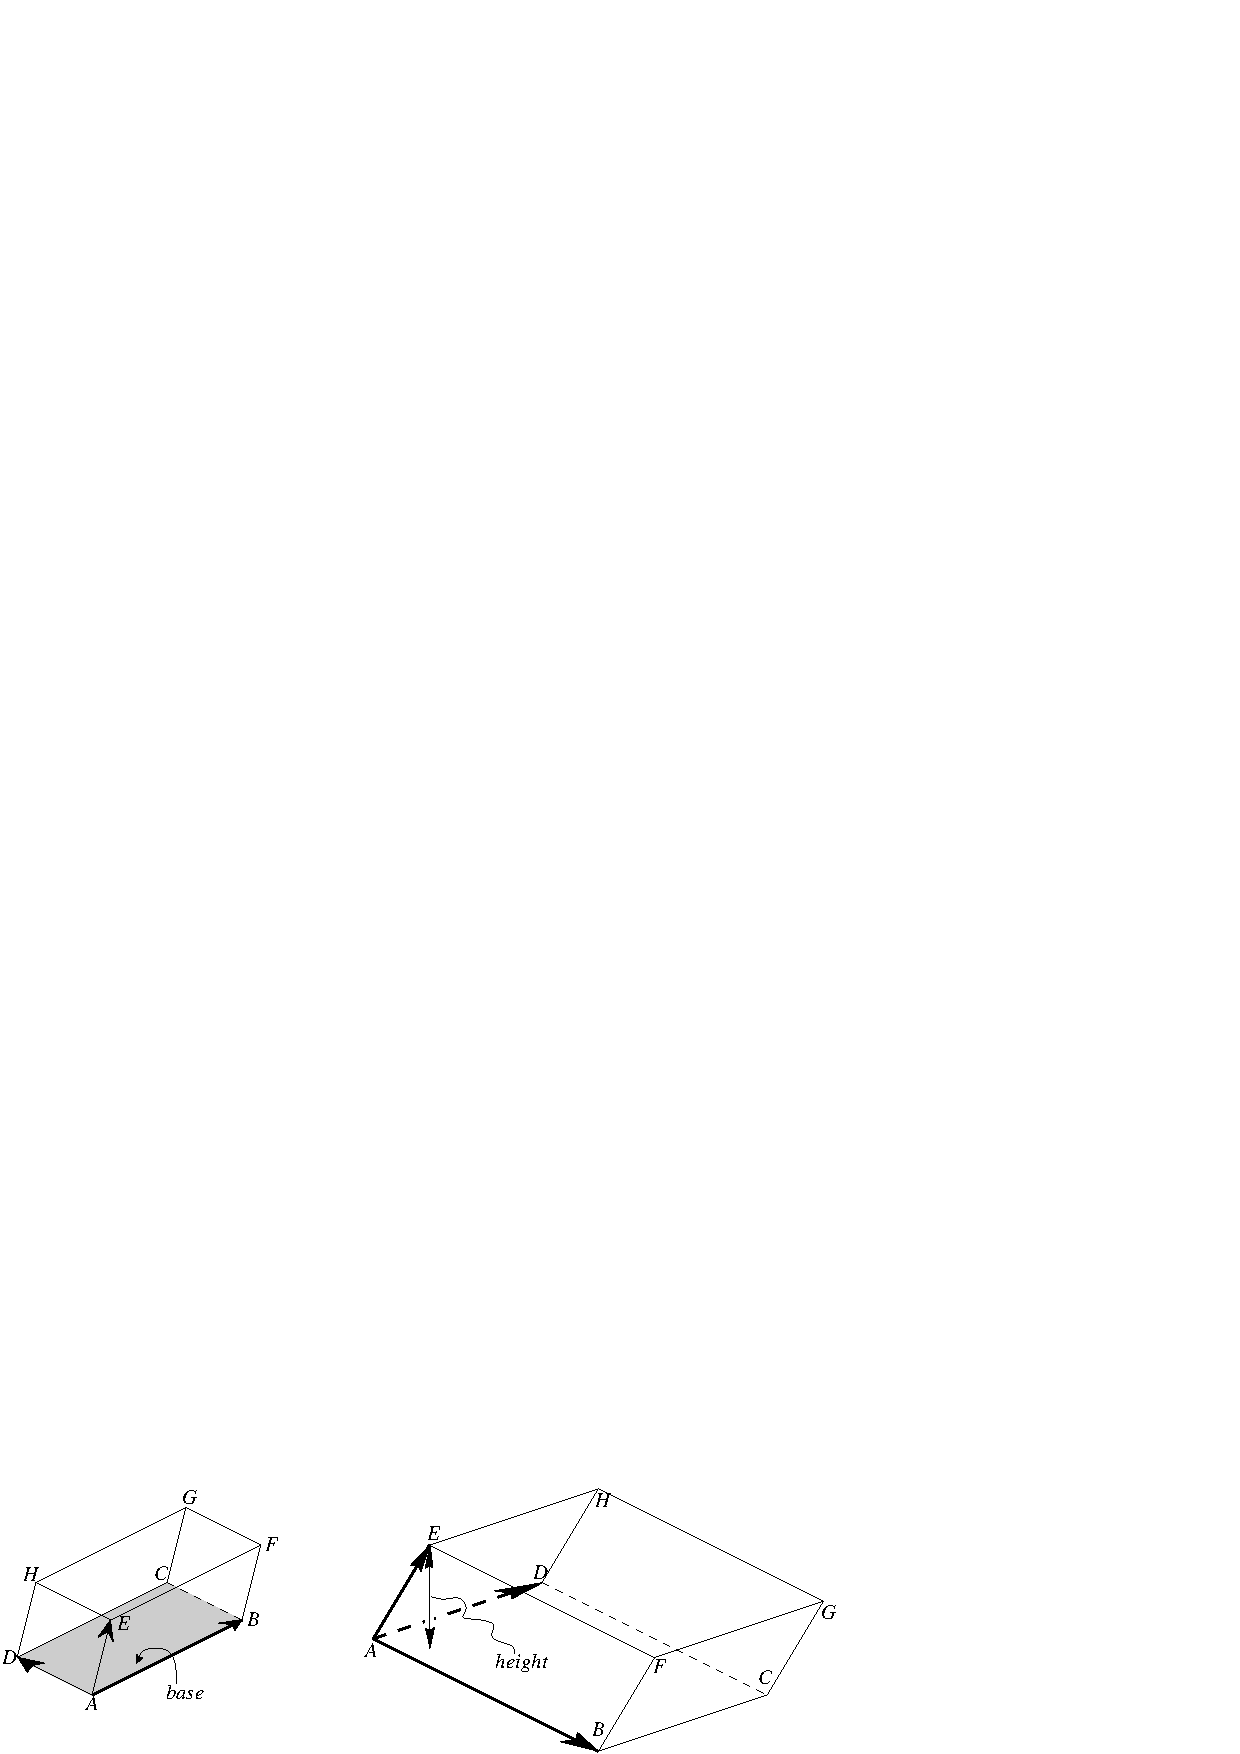
\includegraphics[scale=0.8]{../figures/222/05parallelepiped.pdf}
\end{center}
A \emph{parallelepiped} is a three dimensional body whose sides are
parallelograms. For instance, a cube is an example of a
parallelepiped; a rectangular block (whose faces are rectangles,
meeting at right angles) is also a parallelepiped. Any parallelepiped
has 8 vertices (corner points), 12 edges and 6 faces.

Let $\parppd ABCDEFGH$ be a parallelepiped. If we call one of the
faces, say $ABCD$, the base of the parallelepiped, then the other face
$EFGH$ is parallel to the base. The \emph{height of the
parallelepiped} is the distance from any point in $EFGH$ to the
base, e.g.~to compute the height of $\parppd ABCDEFGH$ one could
compute the distance from the point $E$ (or $F$, or $G$, or $H$) to
the plane through $ABCD$.

The volume of the parallelepiped $\parppd ABCDEFGH$ is given by the
formula
\[
  \text{Volume }\parppd ABCDEFGH = \text{Area of base} \times
  \text{height}.
\]
Since the base is a parallelogram we know its area is given by 
\[
  \text{Area of base} ABCD = \nm{\tpv AB\cp \tpv AD}
\]
We also know that $\vn = \tpv AB\cp \tpv AD$ is a vector perpendicular
to the plane through $ABCD$, i.e.~perpendicular to the base of the
parallelepiped. If we let the angle between the edge $AE$ and the
normal $\vn$ be $\psi$, then the height of the parallelepiped is given
by
\[
  \text{height} = \nm{\tpv AE}\cos\psi.
\]
Therefore the triple product of $\tpv AB, \tpv AD, \tpv AE$ is
\begin{align*}
  \text{Volume }\parppd ABCDEFGH
  &=\text{height} \times \text{Area of base} \\
  &=\nm{\tpv AE}\cos\psi\;\;\nm{\tpv AB\cp\tpv AD},
\end{align*}
i.e.
\[
  \fbox{$\displaystyle
  \text{Volume }\parppd ABCDEFGH
  =\tpv AE\dpp (\tpv AB\cp\tpv AD).$}
\]



\section{Notation} \label{sec:notation} 
When we use vectors to describe the real world it is very important to
distinguish between a point $A$, its position vector $\va = \tpv OA$, and its
coordinates $a_1, a_2, a_3$.    

\begin{itemize}
\item A \emph{point} can be any point in space. For instance, $A$ could be the
  top of the Lincoln statue on Bascom Hill.  That is a well-defined location.

\item To specify the \emph{position vector} for a point we must also specify
  which point we decide to call the origin (the center of the Capitol; or the
  center of the Earth; or the center of the Sun; etc.).  Different choices of
  origins give us different position vectors for the same point.

\item To specify the \emph{coordinates} of the point $A$ we not only need an
  origin, but we also have to specify three perpendicular axes, which we call
  the $x$, $y$, and $z$ axes (or we can give them different names).
\end{itemize}

Given a point in the plane, or in space we can form its position vector. So
associated to a point we have three different mathematical objects: the point,
its position vector and its coordinates.  Table~\ref{tbl:vectornotation}
summarises these different notations.

\begin{table}[b]
  \sffamily\color{darkbluegreen}
  \begin{tabular}{p{140pt}p{200pt}}
    \toprule
    {\bfseries Object} & {\bfseries Notation} \\
    \midrule
    Point&
    Upper case letters, $A$, $B$, etc. \\
    \midrule
    Position vector&
    Lowercase letters with an arrow on top. The position vector
    $\tpv OA$ of the point $A$ should be $\va$, so that letters
    match across changes from upper to lower case.  \\[3ex]
      \midrule
      Coordinates of a point&
      The coordinates of the point $A$ are the same as the components
      of its position vector $\va$: we use lower case letters with a
      subscript to indicate which coordinate we have in mind: $(a_1,
      a_2)$.\\
      \bottomrule
    \end{tabular}
    \caption{The different notations that we have used in this chapter}
    \label{tbl:vectornotation}
\end{table}

\subsection*{Common abuses of notation that should be avoided} 
Sometimes students will write things like
\[
  \va=\vek 3 \\ 1 \\ 2 \tor = 6, \hspace{1in}\text{(\textit{aargh!})}
\]
which really can't be true because $\tvek 3\\1\\2\ttor$ is a vector
and $6$ is a number.   \emph{\color{badgerred}Vectors and numbers are not equal!}

More subtle is the mistake
\[
  \vek 0\\0\\0\tor =0 \qquad\text{\carefulnow}
\]
which looks \textsc{ok}, but it isn't: it's still an equation that
says that some vector and some number are equal. In this case the
vector $\tvek 0\\0\\0\ttor$ is the \emph{zero vector} for which we use
the symbol $\vvv0$. So 
\[
  \vek 0\\0\\0\tor =\vvv0
\]
is correct.


\bigskip





























































\newpage
\section{Problems--Computing and drawing vectors} 
\problemfont

\begin{multicols}{2}
\problem Simplify the following 
\begin{align*}
  \va &= \vek 1\\-2\\3 \tor + 3\vek 0 \\ 1 \\3 \tor; \\
  \vb &=  12\vek 1 \\ 1/3\tor - 3\vek 4 \\ 1\tor; \\
  \vc &= (1+t)\vek 1 \\ 1-t\tor - t\vek 1 \\ -t\tor, \\
  \vd &= t\vek1\\0\\0\tor + t^2\vek0\\-1\\2\tor-\vek0\\0\\1\tor.
\end{align*}

\problem If $\va,\vb, \vc$ are as in the previous problem, then 
which of the following expressions mean anything? Compute those
expressions that are well defined.
\begin{align*}
  \tsubprob& \va+\vb  &\tsubprob& \vb+\vc &\tsubprob& \pi\va \\
  \tsubprob& \vb^2    &\tsubprob& \vb/\vc &\tsubprob& \nm\va+\nm\vb \\
  \tsubprob& \nm\vb^2 &\tsubprob& \vb/\nm\vc &&
\end{align*}

\problem Let $\va =\tvek 1 \\ -2 \\ 2 \ttor$ and $\vb =\tvek 2 \\ -1 \\ 1 \ttor$.
\quad Compute:

\subprob $||\va ||$

\subprob $2\va $

\subprob $||2\va ||^2$

\subprob $\va +\vb $

\subprob $3\va -\vb $




\answer  
(a) $3$ \quad
(b) $\tvek 2 \\ -4 \\ 4 \ttor$  \quad
(c) 36  \quad
(d) $\tvek 3 \\ -3 \\ 3 \ttor$  \quad
(e) $\tvek 1 \\ -5 \\ 5 \ttor$
\endanswer

\problem Let $\vu, \vv,\vw$ be three given vectors, and suppose 
\[
  \va = \vv+\vw,\quad \vb = 2\vu-\vw,\quad \vc = \vu+\vv+\vw.
\]
\subprob Simplify $\vp = \va+3\vb-\vc$ and $\vq = \vc-2 (\vu+\va)$.

\subprob Find numbers $r,s,t$ such that $r\va+s\vb+t\vc=\vu$.

\subprob Find numbers $k,l,m$ such that $k\va+l\vb+m\vc=\vv$.

\problem Prove the Algebraic Properties 
\eqref{eq:vector-addition-cmttve},
\eqref{eq:vector-addition-associative},
\eqref{eq:vector-addition-distrib-1}, and
\eqref{eq:vector-addition-distrib-2} in section
\ref{sec:prop-vect-addit}.

\problem \subprob Does there exist a number $x$ such that 
\[
  \vek 1 \\2 \tor +\vek x \\ x \tor = \vek 2 \\ 1 \tor ?
\]

\subprob Make a drawing of all points $P$ whose position vectors are
given by
\[
  \vp = \vek 1 \\2 \tor +\vek x \\ x \tor.
\]

\subprob Do there exist a numbers $x$ and $y$ such that
\[
  x\vek 1 \\2 \tor + y \vek 1 \\ 1 \tor = \vek 2 \\ 1 \tor ?
\]
\answer 
(a) Since $\vek 1 \\ 2 \tor +\vek x \\ x \tor = \vek 1+x \\ 2+x\tor$ the number
$x$ would have to satisfy both $1+x=2$ and $2+x=1$.  That's impossible, so
there is no such $x$.

(b) No drawing, but $\vp = \vek 1 \\ 2 \tor +\vek x \\ x \tor =
\vek 1\\ 2\tor + x \vek 1\\ 1\tor$ is the parametric representation of a
straight line through the points $(1,2)$ (when $x=0$) and $(2,3)$ (when
$x=1$).

(c) $x$ and $y $ must satisfy $\vek x+y \\ 2x+y\tor = \vek 2\\ 1\tor$.  Solve
$x+y = 2$, $2x+y = 1$ to get $x=-1$, $y=3$.
\endanswer

\problem Given points $A (2,1)$ and $B (-1,4)$ compute the vector 
$\tpv AB$.  \textit{Is $\tpv AB$ a position vector?}
\answer 
Every vector is a position vector.  To see of which point it is the position
vector translate it so its initial point is the origin.

Here $\tpv AB = \vek -3\\ 3 \tor$, so $\tpv AB$ is the position vector of
the point $(-3,3)$.
\endanswer

\problem Given: points $A (2,1)$, $B (3,2)$, $C (4,4)$ and $D 
(5,2)$.  \textit{Is $ABCD$ a parallelogram?}
\answer 
One always labels the vertices of a parallelogram counterclockwise (see
\S\ref{sec:diag-parall}). 

$ABCD$ is a parallelogram if $\tpv AB + \tpv AD = \tpv AC$.  
$\tpv AB = \vek 1\\ 1 \tor$, $\tpv AC = \vek 2\\ 3 \tor$, $\tpv AD = \vek 3\\
1 \tor$.  So $\tpv AB + \tpv AD \ne \tpv AC$, and $ABCD$ is not a
parallelogram.
\endanswer

\problem Given: points $A (0,2,1)$, $B (0,3,2)$, $C (4,1,4)$ and 
$D$.

\subprob If $ABCD$ is a parallelogram, then what are the coordinates of
the point $D$?
\answer 
As in the previous problem, we want $\tpv AB + \tpv AD = \tpv AC$.
If $D$ is the point $(d_1, d_2, d_3)$ then 
$\tpv AB = \vek 0\\ 1\\1 \tor$, 
$\tpv AD = \vek d_1\\ d_2-2 \\ d_3-1\tor$,
$\tpv AC = \vek 4\\ -1\\ 3 \tor$,
so that $\tpv AB + \tpv AD = \tpv AC$ will hold if 
$d_1 = 4$, $d_2 = 0$ and $d_3 = 3$.
\endanswer

\subprob If $ABDC$ is a parallelogram, then what are the coordinates of
the point $D$?
\answer 
Now we want $\tpv AB + \tpv AC = \tpv AD$, so $d_1 = 4$, $d_2 = 2$,
$d_3 = 5$.
\endanswer

\problem \label{pblm:draw-vectors} You are given three points in the 
plane: $A$ has coordinates $(2,3)$, $B$ has coordinates $(-1,2)$ and
$C$ has coordinates $(4,-1)$.

\subprob Compute the vectors $\tpv AB$, $\tpv BA$, $\tpv AC$, $\tpv CA$, $\tpv
BC$ and $\tpv CB$.

\subprob Find the points $P, Q, R$ and $S$ whose position vectors are $\tpv AB$,
$\tpv BA$, $\tpv AC$, and $\tpv BC$, respectively.  \textit{Make a precise
drawing in figure~\ref{fig:draw-vectors-here}.}


\problem \label{pblm:draw-v-plus-w} Have a look at 
figure~\ref{fig:draw-v-plus-w}

\subprob Draw the vectors $2\vv+\tfrac12\vw$, $-\tfrac12\vv+\vw$,
and $\tfrac32\vv-\tfrac12\vw$

\subprob Find real numbers $s,t$ such that $s\vv+t\vw=\va$.

\subprob Find real numbers $p,q$ such that $p\vv+q\vw=\vb$.

\subprob Find real numbers $k,l,m,n$ such that $ \vv = k\va+l\vb$, and
$\vw = m\va+n\vw $.
\end{multicols}


\begin{figure}[ht]
  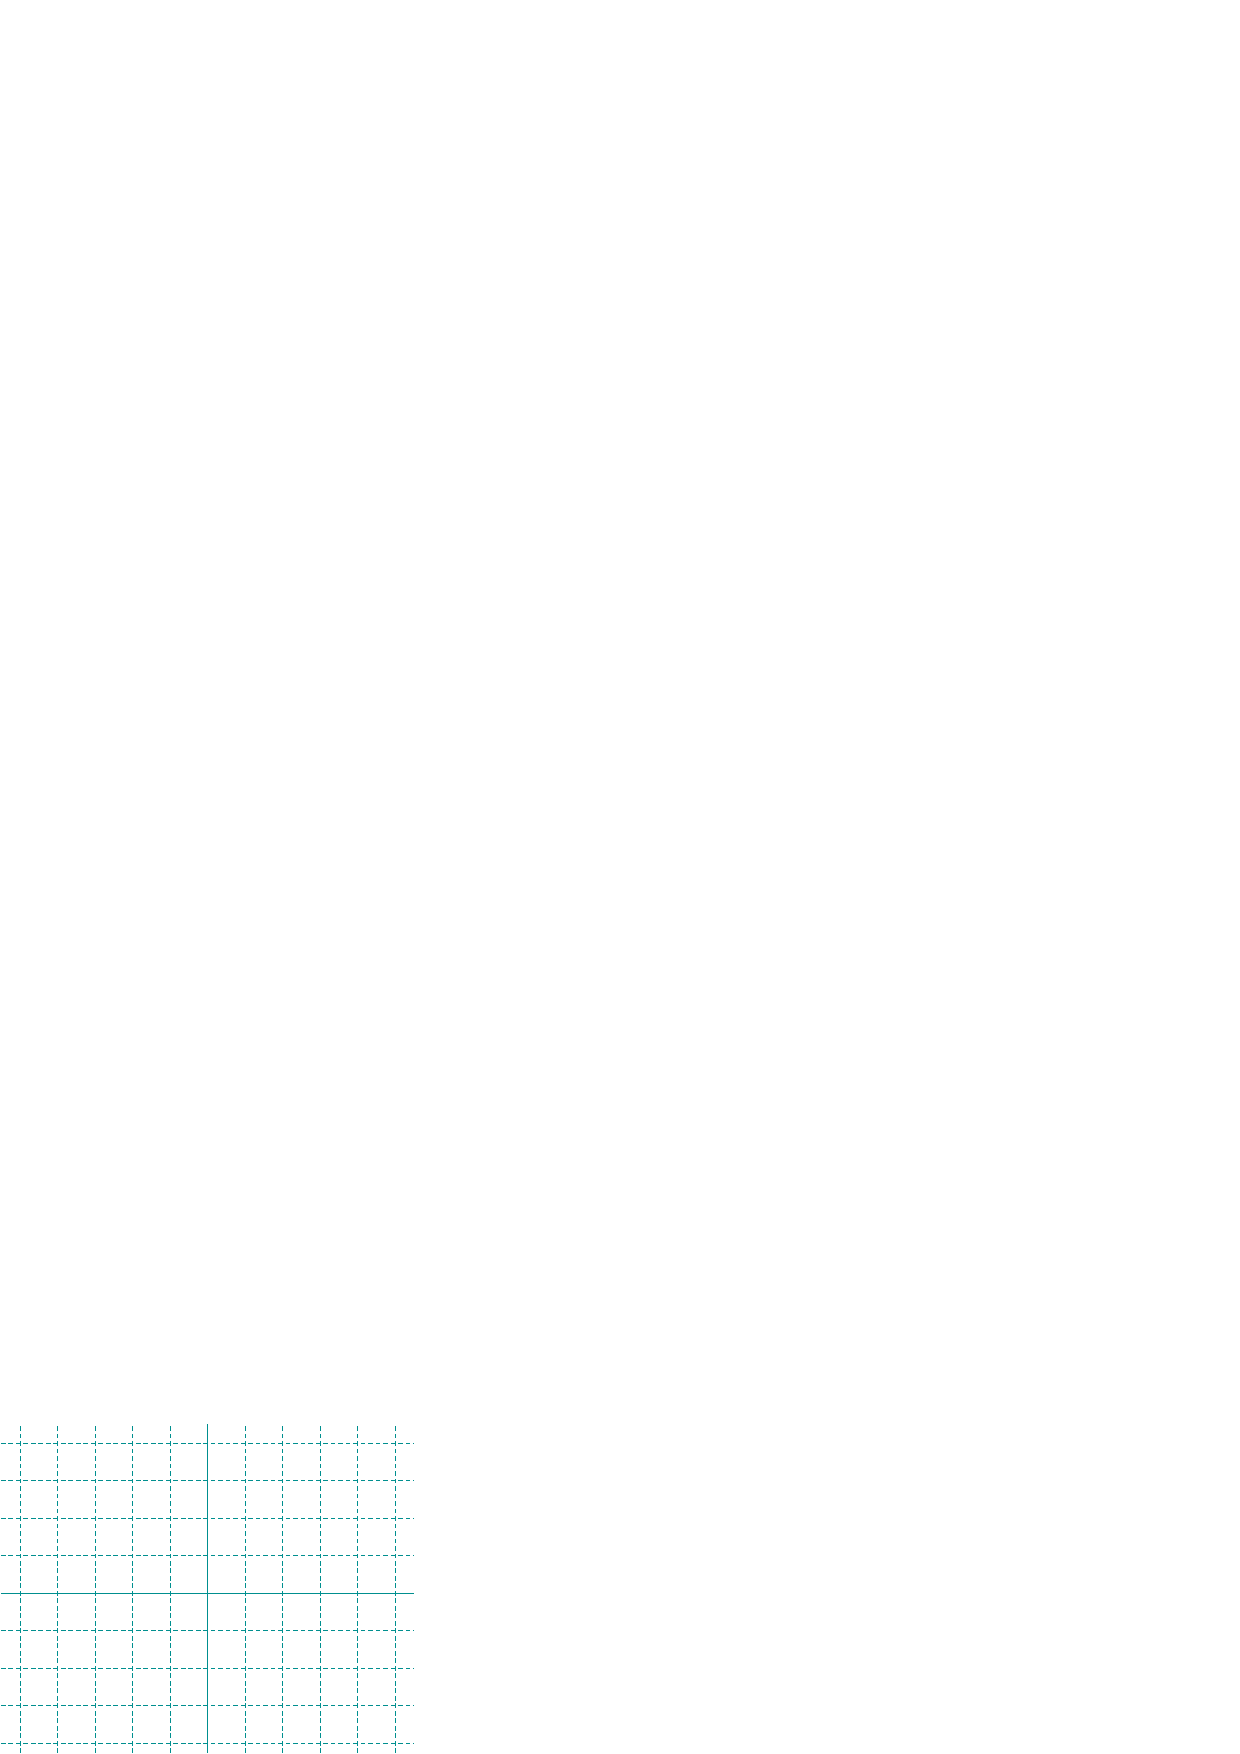
\includegraphics{05graph-paper.pdf}
  \caption{Your drawing for problem \ref{pblm:draw-vectors}}
  \label{fig:draw-vectors-here}
\end{figure}


\begin{figure}[hb]
  \input{../figures/222/05drawsome.pdf_tex}
  \caption{Drawing for problem \ref{pblm:draw-v-plus-w}}
  \label{fig:draw-v-plus-w}
\end{figure}


\begin{center}
  \includegraphics{05parametricline.pdf}
\end{center}

\section{Problems--Parametric equations for a line}  
\begin{multicols}{2}

\problem In the figure above draw the points whose position vectors are 
given by $\vx=\va+t (\vb-\va)$ for $t= 0,1,\frac13,\frac34, -1, 2$.
(as always, $\va=\tpv OA$, etc.)

\problem In the figure above also draw the points whose position 
vector are given by $\vx=\vb+s (\va-\vb)$ for $s= 0,1,\frac13,\frac34,
-1, 2$.

\problem \subprob  Find a parametric equation for the line $\ell$ 
through the points $A (3,0,1)$ and $B (2,1,2)$.

\subprob  Where does $\ell$ intersect the coordinate planes?
\answer 
(a)
$\vx = \vek 3\\ 0\\1 \tor + t \vek -1\\ 1\\1 \tor = \vek 3-t\\ t\\ 1+t \tor$.  

(b) Intersection with $xy$ plane when $z=0$, i.e.\ when $t=-1$, at $(4, -1,
0)$.
Intersection with $xz$ plane when $y=0$, when $t=0$, at $(3,0,1)$ (i.e.\ at
$A$).  Intersection with $yz$ plane when $x=0$, when $t=3$, at $(0, 3, 4)$. 
\endanswer

\problem 
\subprob  Find a parametric equation for the line which contains
the two vectors 

\medskip
$\va =\tvek 2 \\ 3 \\ 1 \ttor$ and $\vb =\tvek 3 \\ 2 \\ 3 \ttor$.

\subprob  The vector $\vc =
\left(\begin{array}{c}
  c_1 \\
  1\\
  c_3 \\
\end{array}\right)$ is on this line.  What
is $\vc $?



\answer  
(a) $\vec{L}[t]=\tvek 2 \\ 3 \\ 1 \ttor+t\tvek 1 \\ -1 \\ 2 \ttor$
\par (b) $\tvek 4 \\ 1 \\ 5 \ttor$
\endanswer



\problem \groupproblem  Consider a triangle $ABC$ and let $\va,\vb,\vc$ be the 
position vectors of $A,B$, and $C$.

\subprob  Compute the position vector of the midpoint $P$ of the line
segment $BC$. Also compute the position vectors of the midpoints $Q$
of $AC$ and $R$ of $AB$. (Make a drawing.)

\subprob  Let $M$ be the point on the line segment $AP$ which is twice
as far from $A$ as it is from $P$. Find the position vector of $M$.

\subprob  Show that $M$ also lies on the line segments $BQ$ and $CR$.

\answer 
(a) $\vp = (\vb+\vc)/2$,  $\vq = (\va+\vc)/2$, $\vr = (\va+\vb)/2$.

(b) $\vm = \va + \frac23(\vp-\va)$  (See Figure \ref{fig:line-through-AB},
with $AX$ twice as long as $XB$).  Simplify to get
$\vm = \frac13\va + \frac13\vb + \frac13\vc$.

(c) Hint : find the point $N$ on the line segment $BQ$ which is twice as far
from $B$ as it is from $Q$.  If you compute this carefully you will find that
$M=N$. 
\endanswer


\problem \groupproblem  Let $ABCD$ be a tetrahedron, and let $\va,\vb,\vc,\vd$ be the 
position vectors of the points $A,B,C,D$.

\subprob Find position vectors of the midpoint $P$ of $AB$, the
midpoint $Q$ of $CD$ and the midpoint $M$ of $PQ$.

\subprob Find position vectors of the midpoint $R$ of $BC$, the
midpoint $S$ of $AD$ and the midpoint $N$ of $RS$.

\begin{center}
  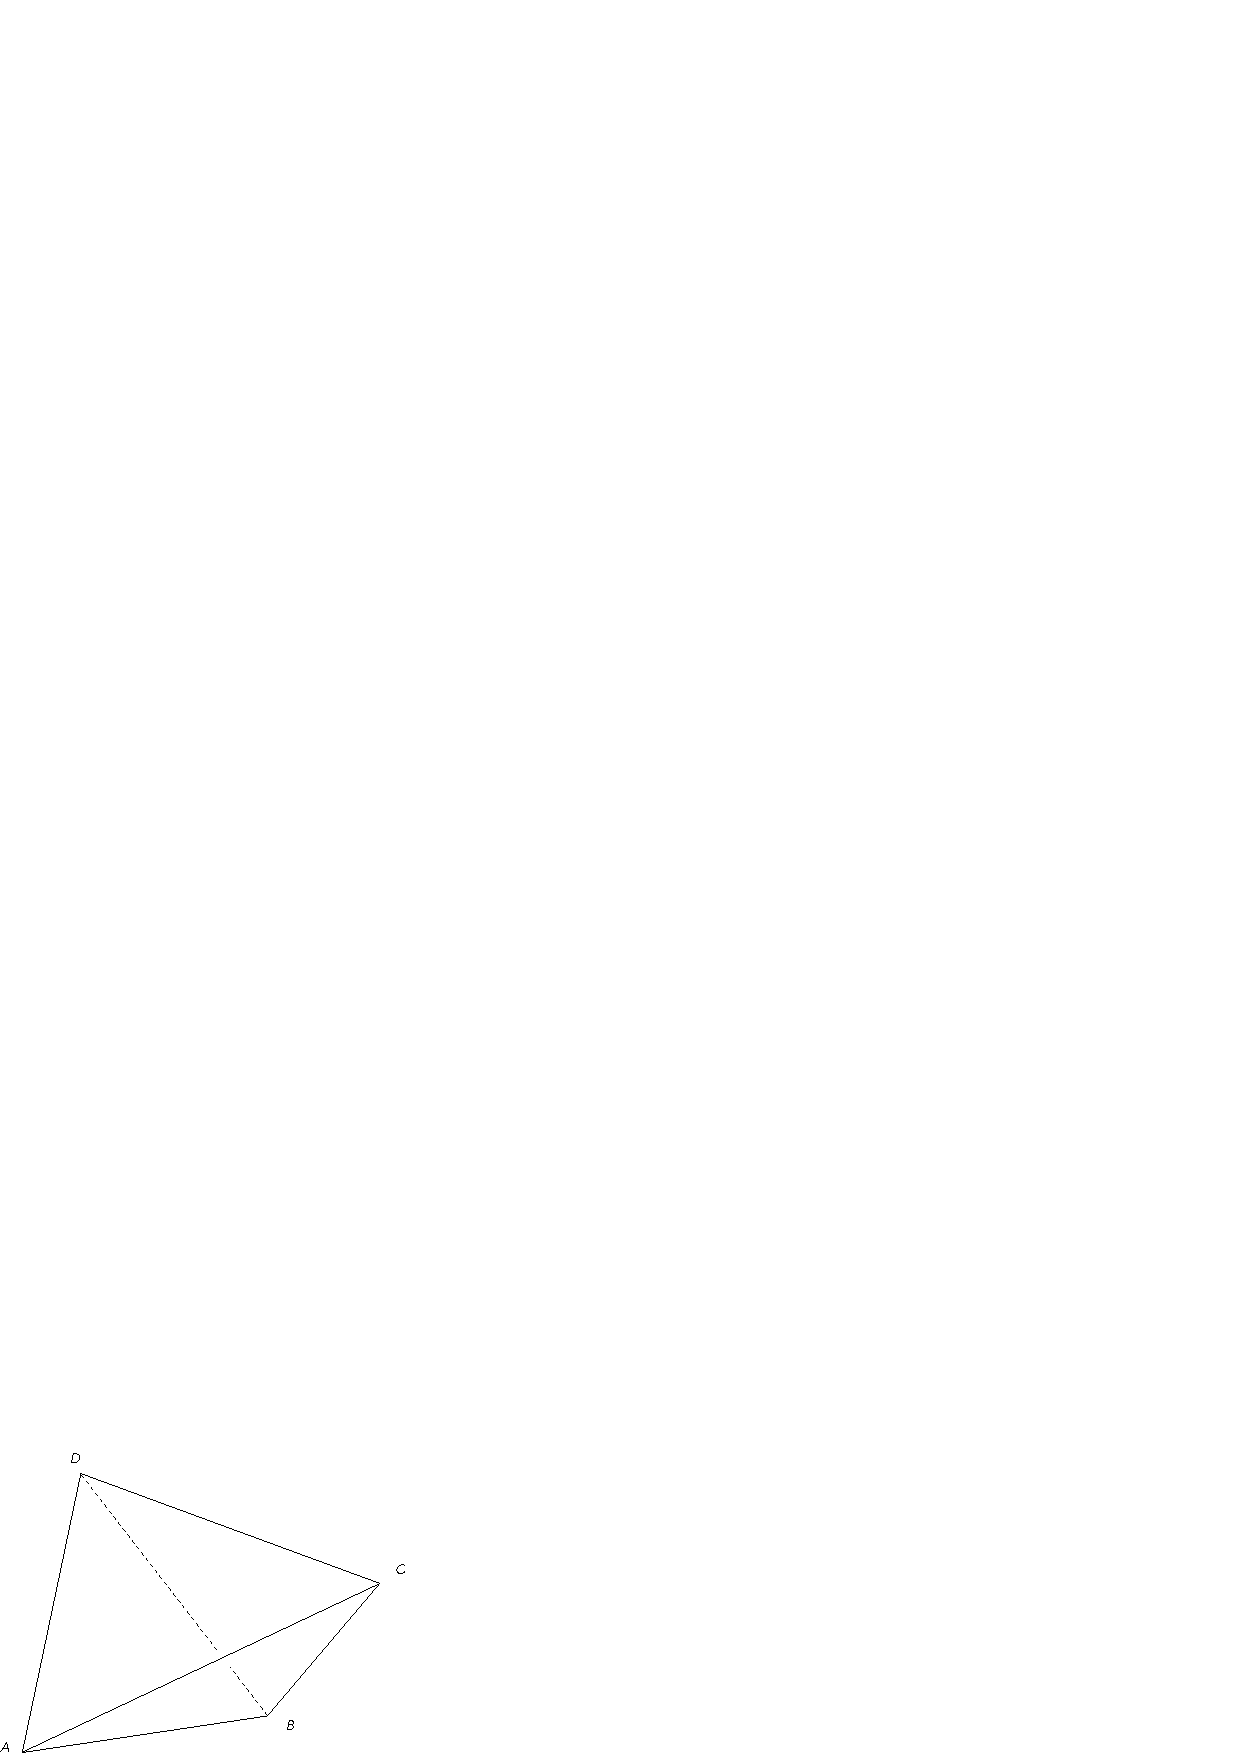
\includegraphics{05tetrahedron.pdf}
\end{center}
\end{multicols}

\section{Problems--Orthogonal decomposition\\of one vector with respect to another}  

\begin{multicols}{2}
\problem Given the vectors $\va=\tvek 2\\1\\3\ttor$ and $\vb=\tvek 1 
\\ 1 \\ 0\ttor$ find $\va^\pll$, $\va^\perp$, $\vb^\pll$, $\vb^\perp$
for which
\[
  \va=\va^\pll+\va^\perp, \text{ with }a^\pll\pll\vb, a^\perp\perp\vb, 
\]
and
\[
  \vb=\vb^\pll+\vb^\perp, \text{ with }b^\pll\pll\va, b^\perp\perp\va. 
\]
\answer 
To decompose $\vb$ set $\vb= \vb_\perp+\vb_\pll$, with $\vb_\pll = t\va$ for
some number $t$.  Take the dot product with $\va$ on both sides and you get
$\va\dpp\vb = t\|\va\|^2$, whence $3 = 14 t$ and $t=\frac3{14}$.  Therefore
\[
  \vb_\pll = \frac{3}{14}\va, \qquad \vb_\perp = \vb-\frac{3}{14}\va.
\]
To find $\vb_\pll$ and $\vb-\perp$ you now substitute the given values for
$\va$ and $\vb$.


The same procedure leads to $\va_\perp$ and $\va_\pll$:
$\va_\pll = \frac{3}{2}\vb$, $\va_\perp = \va - \frac32\vb$.
\endanswer


\problem Bruce left his backpack on a hill, which in some coordinate system 
happens to be the line with equation $12x_1 + 5x_2 = 130$.

The force exerted by gravity on the backpack is $\vf_{\rm grav}=\tvek 0 \\
-mg\ttor$. Decompose this force into a part perpendicular to the hill, and a
part parallel to the hill.
\begin{center}
  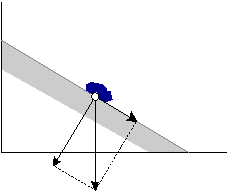
\includegraphics{05bruce-backpack.pdf}
\end{center}
\answer 
This problem is of the same type as the previous one, namely we have to
decompose one vector as the sum of a vector perpendicular and a vector
parallel to the hill's surface.  The only difference is that we are not given
the normal to the hill so we have to find it ourselves.  The equation of the
hill is $12x_1 + 5x_2 = 130$ so the vector $\vn = \tvek 12\\ 5\ttor$ is a
normal.

The problem now asks us to write $\vf_{\rm grav} = \vf_\perp + \vf_\pll$,
where $\vf_\perp = t\vn$ is perpendicular to the surface of the hill, and
$\vf_\pll$ id parallel to the surface.  

Take the dot product with $\vn$, and you find $t\|\vn\|^2 =
\vn\dpp\vf_{\rm grav} \implies 169t = -5mg \implies t=-\frac{5}{169}mg$.
Therefore 
\[
  \vf_\perp = -\frac{5}{169}mg\vek12 \\5\tor
  =\vek -\frac{60}{169}mg \\ -\frac{25}{169}mg\tor,
  \qquad
  \vf_\pll = \vf_{\rm grav} - \vf_\perp
  = \vek -\frac{60}{169}mg \\ \frac{144}{169}mg\tor,
\]
\endanswer

\problem An eraser is lying on the plane $\cP$ with equation 
$x_1+3x_2+x_3 = 6$. Gravity pulls the eraser down, and exerts a force
given by
\[
  \vf_{\rm grav} = \vek 0\\ 0\\ -mg\tor.
\]

\subprob  Find a normal $\vn$ for the plane $\cP$.

\subprob  Decompose the force $\vf$ into a part perpendicular to the plane $\cP$ and a
part perpendicular to $\vn$.
\end{multicols}

\section{Problems--The dot product}  

\begin{multicols}{2}
\problem 
\subprob  Simplify $\nm{\va-\vb}^2$.

\subprob  Simplify $\nm{2\va-\vb}^2$. 

\subprob  If $\va$ has length 3, $\vb$ has length $7$ and
$\va\dpp\vb=-2$, then compute $\nm{\va+\vb}$, $\nm{\va-\vb}$ and
$\nm{2\va-\vb}$.
\answer 
$\|\va-\vb\|^2 = \|\va\|^2 - 2\va\dpp\vb + \|\vb\|^2$;
$\|2\va-\vb\|^2 = 4\|\va\|^2 - 4\va\dpp\vb + \|\vb\|^2$;
$\nm{\va+\vb} = \sqrt{54}$, $\nm{\va-\vb} = \sqrt{62}$ and
$\nm{2\va-\vb}=\sqrt{130}$.
\endanswer

\problem Simplify $(\va+\vb)\dpp (\va-\vb)$. 

\problem Find the lengths of the sides, and the angles in the triangle 
$ABC$ whose vertices are $A (2,1)$, $B(3,2)$, and $C(1,4)$.

\answer 
Compute $\tpv AB = -\tpv BA = \vek 1\\ 1\tor$,
$\tpv BC = -\tpv CB = \vek -2 \\ 2 \tor$,
$\tpv AC = -\tpv CA = \vek -1 \\ 3 \tor$.
Hence
$\|\tpv AB\| = \sqrt{2}$,
$\|\tpv BC\| = \sqrt{8} = 2\sqrt{2}$,
$\|\tpv AC\| = \sqrt{10}$.

And also $\tpv AB\dpp \tpv AC = 2 \implies \cos \angle A =
\frac{\tpv AB\dpp \tpv AC}{\|\tpv AB\|\,\|\tpv AC\|} =
\frac{2}{\sqrt{20}} = \frac{1}{\sqrt{5}}$.

A similar calculation gives $\cos \angle B = 0$ so we have a right triangle;
and $\cos\angle C = \frac{2}{\sqrt{5}}$.
\endanswer

\problem \groupproblem  
Given: $A(1,1)$, $B(3,2)$ and a point $C$ which lies on the
line with parametric equation $\vc=\tvek 0\\3 \ttor + t\tvek
1\\-1\ttor$. If $\triangle ABC$ is a right triangle, then where is
$C$? (There are three possible answers, depending on whether you
assume $A$, $B$ or $C$ is the right angle.)
\answer 
$\tpv AB = \tvek2\\1\ttor$,
$\tpv AC = \tvek t-1\\ 2-t\ttor$,
$\tpv BC = \tvek t-3 \\1-t\ttor$.

If the right angle is at $A$ then $\tpv AB \dpp \tpv AC = 0$, so that
we must solve $2(t-1) + (2-t) = 0$. Solution: $t=0$, and $C = (0,3)$.

If the right angle is at $B$ then $\tpv AB \dpp \tpv BC = 0$, so that
we must solve $2(t-3) + (1-t) = 0$. Solution: $t=5$, and $C = (5, -2)$.

If the right angle is at $C$ then $\tpv AC \dpp \tpv BC = 0$, so that
we must solve $(t-1)(t-3) + (2-t)(1-t) = 0$. Note that this case is
different in that we get a quadratic equation, and in that there are two
solutions, $t=1$, $t=\frac52$.

This is a complete solution of the problem, but it turns out that there is a
nice picture of the solution, and that the four different points $C$ we find
are connected with the circle whose diameter is the line segment $AB$:
\begin{center}
  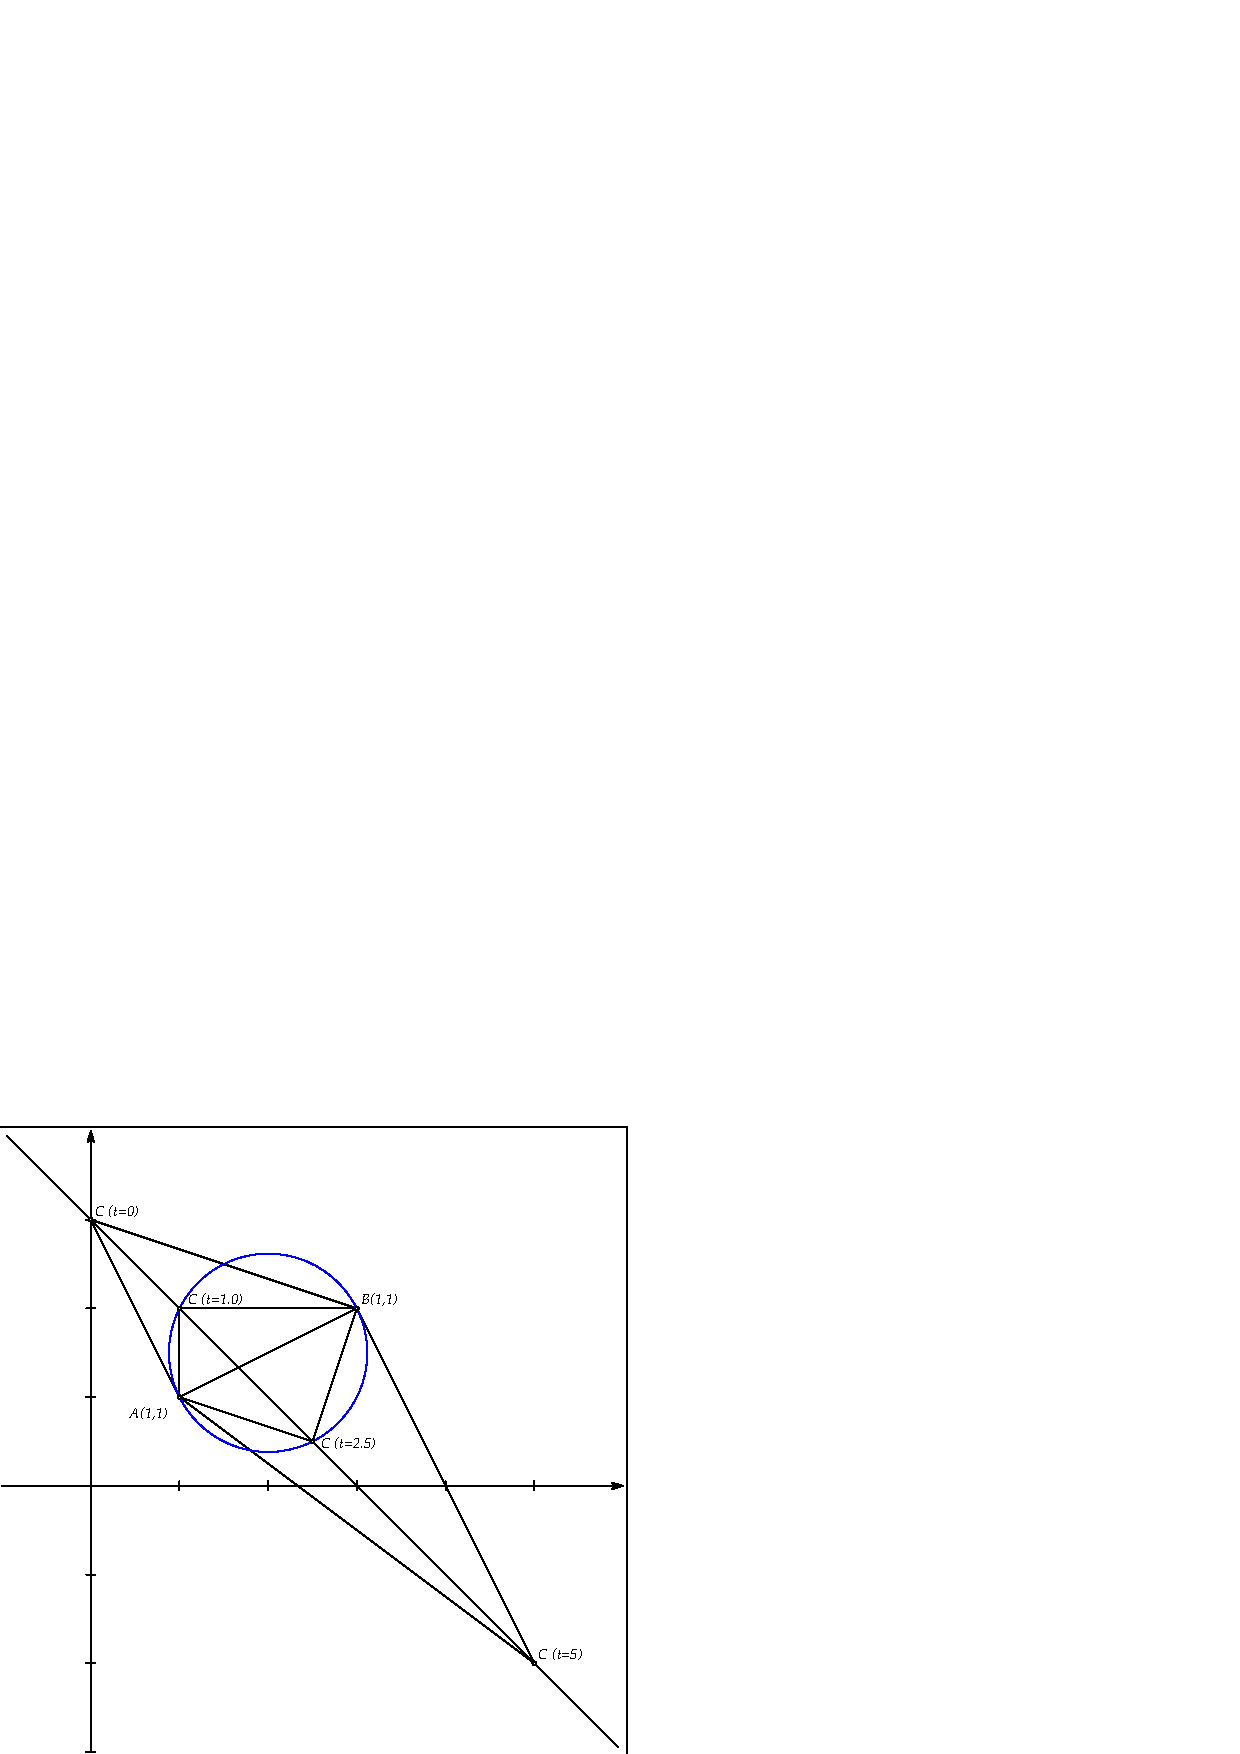
\includegraphics{05rightangle-problem.pdf}
\end{center}
\endanswer

\problem  
\subprob Find the defining equation and a normal vector $\vn$ for the
line $\ell$ which is the graph of $y=1+\frac12x$.
\answer 
$\ell$ has defining equation $-\frac12 x + y = 1$ which is of the form
$\vn\dpp\vx = $constant if you choose $\vn = \tvek-1/2 \\ 1\ttor$.
\endanswer


\subprob What is the distance from the origin to $\ell$?
\answer 
The distance to the point $D$ with position vector $\vd$ from the line
$\ell$ is $\frac{\vn\dpp(\vd-\va)}{\|\vn\|}$ where $\va$ is the position
vector of any point on the line.  In our case $\vd = \vvv0$
and the point $A(0,1)$, $\va = \tpv OA = \tvek 0\\1\ttor$, is on the line.
So the distance to the origin from the line is $\dfrac{-\vn\dpp\va}{\|\vn\|}
= \dfrac{1}{\sqrt{(1/2)^2 + 1^2}} = 2/\sqrt{5}$.
\endanswer

\subprob Answer the same two questions for the line $m$ which is the
graph of $y=2-3x$.
\answer 
$3x+y=2$, normal vector is $\vm = \tvek3\\1\ttor$. 
\endanswer

\subprob What is the angle between $\ell$ and $m$?
\answer 
Angle between $\ell$ and $m$ is the angle $\theta$ between their normals,
whose cosine is $\cos \theta = \frac{\vn\dpp\vm}{\|\vn\|\,\|\vm\|} =
\frac{-1/2}{\sqrt{5/4}\sqrt{10}} = -\frac{1}{\sqrt{50} }=
-\frac{1}{10}\sqrt{2}$.
\endanswer

\problem Let $\ell$ and $m $ be the lines with parametrizations 
\begin{align*}
  \ell:&\; \vx=\vek 2 \\ 0 \tor + t \vek 1 \\ 2 \tor ,\\
  m:& \; \vx = \vek 0 \\ -1 \tor + s\vek -2 \\ 3 \tor
\end{align*}
Where do they intersect, and find the angle between $\ell$ and $m$.

\problem Let $\ell$ and $m $ be the lines with parametrizations 
\begin{align*}
  \ell:&\; \vx=\vek 2 \\ 1 \\-4 \tor + t \vek 1 \\ 2 \\0 \tor , \\
  m:& \; \vx = \vek 0\\1 \\ -1 \tor + s\vek -2 \\0 \\ 3 \tor
\end{align*}
Do $\ell$ and $m$ intersect? Find the angle between $\ell$ and $m$.



\problem Let $\ell$ and $m $ be the lines with parametrizations 
\begin{align*}
  \ell:&\; \vx=\vek 2 \\ \alpha \\1 \tor + t \vek 1 \\ 2 \\0 \tor ,\\
  m:&\; \vx = \vek 0\\1 \\ -1 \tor + s\vek -2 \\0 \\ 3 \tor
\end{align*}
Here $\alpha$ is some unknown number. 

If it is known that the lines $\ell$ and $m$ intersect, what can you
say about $\alpha$?
\end{multicols}

\section{Problems--The cross product}  


\begin{multicols}{2}
\problem Compute the following cross products 

\subprob \(\DS \vek 3\\1\\2\tor \cp \vek 3\\2\\1\tor \)

\subprob \(\DS \vek 12\\-71\\3\tfrac12\tor \cp \vek 12\\-71\\3\tfrac12\tor \)

\subprob \(\DS \vek 1\\0\\0\tor \cp \vek 1\\1\\0\tor \)

\subprob \(\DS \vek \surd2\\1\\0\tor \cp \vek 0\\\surd2\\0\tor \)

\problem Compute the following cross products 

\subprob \(\DS \vi\cp (\vi+\vj) \)

\subprob \(\DS (\sqrt2\vi+\vj)\cp \sqrt2\vj \)

\subprob \(\DS (2\vi+\vk)\cp (\vj-\vk) \)

\subprob \(\DS (\cos\theta\vi+\sin\theta\vk)\cp (\sin\theta\vi-\cos\theta\vk)\)

\problem 
\subprob Simplify $(\va+\vb)\cp (\va+\vb)$.
\answer 
$\vvv0$ (the cross product of any vector with itself is the zero vector).
\endanswer

\subprob Simplify $(\va-\vb)\cp (\va-\vb)$.

\subprob Simplify $(\va+\vb)\cp (\va-\vb)$.
\answer 
$(\va+\vb)\cp (\va-\vb) = \va\cp\va +\vb\cp\va - \va\cp\vb - \vb\cp\vb =
-2\va\cp\vb$.
\endanswer

\problem \textit{True or False: } If $\va\cp\vb=\vc\cp\vb$ and 
$\vb\neq\vvv0$ then $\va=\vc$?
\answer 
Not true.  For instance, the vector $\vc$ could be $\vc = \va+\vb$, and
$\va\cp\vb$ would be the same as $\vc\cp\vb$.
\endanswer

\problem \groupproblem  Given $A(2,0,0)$, $B(0,0,2)$ and $C(2,2,2)$. Let $\cP$ be the 
plane through $A$, $B$ and $C$.

\subprob Find a normal vector for $\cP$.
\answer 
A possible normal vector is $\vn = \tpv AB \cp \tpv AC = \tvek-4\\4\\-4\ttor$.
Any (non zero) multiple of this vector is also a valid normal.  The nicest would
be $\frac14\vn = \tvek-1\\1\\-1\ttor$.
\endanswer

\subprob Find a defining equation for $\cP$.
\answer 
$\vn\dpp(\vx-\va) = 0$, or $\vn\dpp\vx = \vn\dpp\va$.  Using $\vn$ and
$\va$ from the first part we get $-4x_1 + 4x_2 -4x_3 = -8$.  Here you could
replace $\va$ by either $\vb$ or $\vc$. (Make sure you understand why; if you
don't think about it, then ask someone).
\endanswer

\subprob What is the distance from $D(0,2,0)$ to $\cP$? What is the
distance from the origin $O(0,0,0)$ to $\cP$?
\answer 
Distance from $D$ to $\cP$ is $\frac{\vn\dpp(\vd-\va)}{\|\vn\|} =
4/\sqrt{3} = \frac43\sqrt{3}$.  There are many valid choices of normal
$\vn$ in part (i) of this problem, but they all give the same answer here.

Distance from $O$ to $\cP$ is $\frac{\vn\dpp(\vvv0-\va)}{\|\vn\|} =
\frac23\sqrt{3}$.
\endanswer

\subprob Do $D$ and $O$ lie on the same side of $\cP$?
\answer 
Since $\vn\dpp(\vvv0-\va)$ and $\vn\dpp(\vd-\va)$ have the same sign the point
$D$ and the origin lie on the same side of the plane $\cP$.
\endanswer

\subprob Find the area of the triangle $ABC$.
\answer 
The area of the triangle is $\frac12\|\tpv AB\cp\tpv AC\| = 2\sqrt{3}$.
\endanswer

\subprob Where does the plane $\cP$ intersect the three coordinate
axes?
\answer 
Intersection with $x$ axis is $A$, the intersection with $y$-axis occurs at
$(0,-2,0)$ and the intersection with the $z$-axis is $B$.
\endanswer


\problem 
\subprob Does $D(2,1,3)$ lie on the plane $\cP$ through the points
$A(-1,0,0)$, $B(0,2,1)$ and $C(0,3,0)$?
\answer 
Since $\vn = \tpv AB\cp\tpv AC = \tvek-3\\1\\1\ttor$ the plane through
$A,B,C$ has defining equation $-3x+y+z = 3$.  The coordinates $(2,1,3)$ of
$D$ do not satisfy this equation, so $D$ is not on the plane $ABC$.
\endanswer

\subprob The point $E(1,1,\alpha)$ lies on $\cP$. What is $\alpha$?
\answer 
If $E$ is on the plane through $A,B,C$ then the coordinates of $E$ satisfy the
defining equation of this plane, so that $-3\cdot1+1\cdot1+1\cdot\alpha = 3$.
This implies $\alpha=5$.
\endanswer

\problem Given points $A(1,-1,1)$, $B(2,0,1)$ and $C(1,2,0)$. 

\subprob Where is the point $D$ which makes $ABCD$ into a parallelogram?
\answer 
If $ABCD$ is a parallelogram then the vertices of the parallelogram are labeled
$A$, $B$, $C$, $D$ as you go around the parallelogram in a counterclockwise
fashion. See the figure in \S43.2.

Then $\tpv AB + \tpv AD = \tpv AC$.  Starting from this equation there
are now two ways to solve this problem.

\textbf{(first solution)}  If $D$ is the point $(d_1, d_2, d_3)$ then $\tpv AD =
\tvek d_1-1 \\d_2+1\\d_3-1\ttor$, while $\tpv AB = \tvek1\\1\\0\ttor$ and $\tpv
AC = \tvek0\\3\\-1\ttor$. Hence $\tpv AB + \tpv AD = \tpv AC$ implies
$\tvek d_1 \\d_2+2 \\d_3-1\ttor = \tvek0\\3\\-1\ttor$, and thus
$d_1 = 0$, $d_2 = 1$ and $d_3 = 0$.

\textbf{(second solution)} Let $\va, \vb, \vc, \vd$ be the position vectors of $A,B,C,D$.
Then $\tpv AB = \vb-\va$, etc.\ and $\tpv AB + \tpv AD = \tpv AC$ is equivalent
to $\vb-\va + \vd-\va = \vc-\va$.  Since we know $\va, \vb, \vc$ we can solve
for $\vd$ and we get
$\vd = \vc-\vb+\va = \tvek1\\-1\\1\ttor - \tvek2\\0\\1\ttor + \tvek1\\2\\0\ttor
= \tvek0\\1\\0\ttor$.
\endanswer

\subprob What is the area of the parallelogram $ABCD$?
\answer 
The area of the parallelogram $ABCD$ is $\|\tpv AB \cp \tpv AD\| =
\left\|\tvek-1\\1\\3\ttor\right\| = \sqrt{11}$.
\endanswer

\subprob Find a defining equation for the plane $\cP$ containing the
parallelogram $ABCD$.
\answer 
In the previous part we computed $\tpv AB \cp \tpv AD = \tvek-1\\1\\3\ttor$, so
this is a normal to the plane containing $A,B,D$.  The defining equation for
that plane is $-x+y+3z = 1$.  Since $ABCD$ is a parallelogram any plane
containing $ABD$ automatically contains $C$.
\endanswer

\subprob Where does $\cP$ intersect the coordinate axes?
\answer 
$(-1,0,0)$, $(0,1,0)$, $(0,0,\frac{1}{3})$.
\endanswer

\problem Given points $A(1,0,0)$, $B(0,2,0)$ and $D(-1,0,1)$ and 
$E(0,0,2)$.

\subprob If $\mathfrak P=\parppd ABCDEFGH$ is a parallelepiped, then
where are the points $C,F,G$ and $H$?
\answer Here is the picture of the parallelepiped (which you can also find on 
page 103):
\begin{center}
  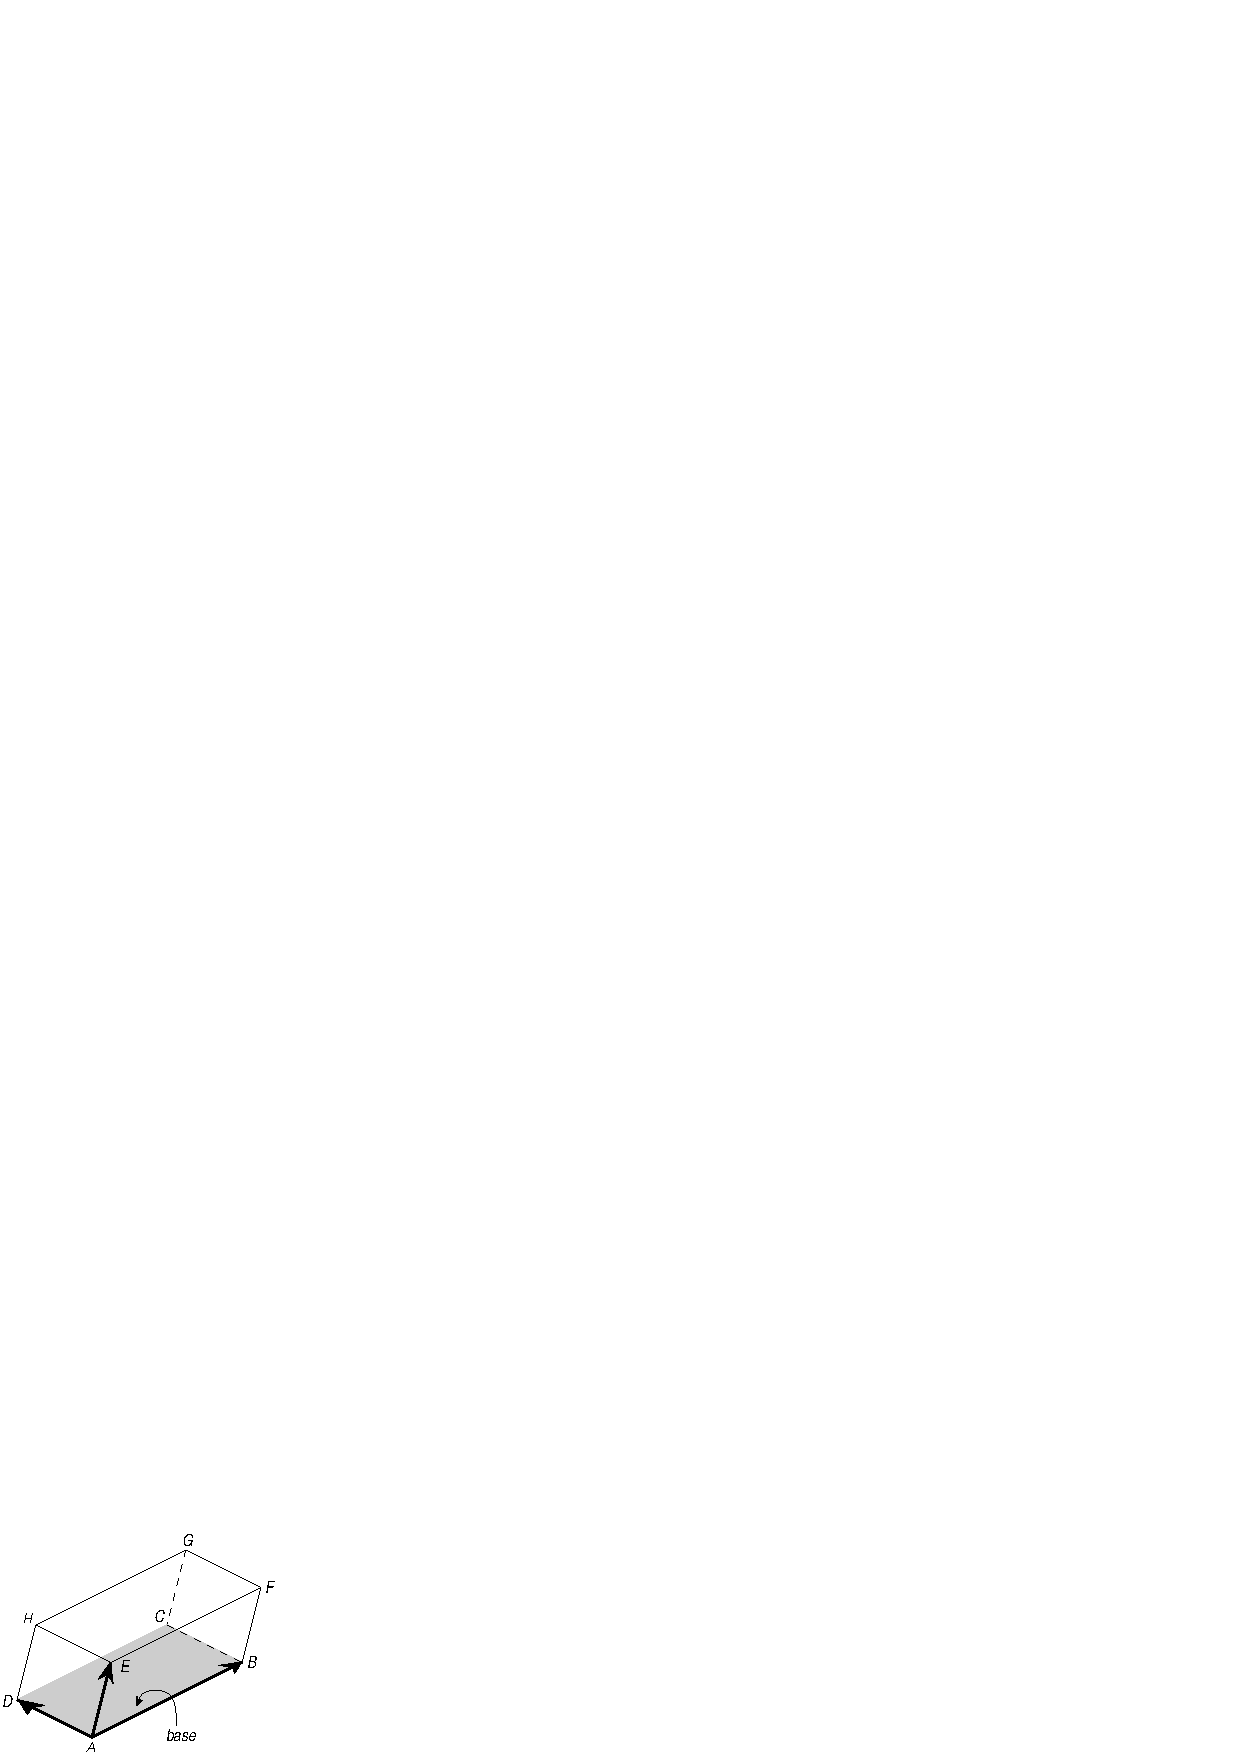
\includegraphics{05parallelepiped2.pdf}
\end{center}
Knowing the points $A, B, D$ we get $\tpv AB = \tvek-1\\2\\0\ttor$,
$\tpv AD = \tvek-2\\0\\1\ttor$.  Also, since $\parppd EFGHABCD$ is a
parallelepiped, we know that all its faces are parallelogram, and thus $\tpv EF
= \tpv AB$, etc.  Hence: we find these coordinates for the points $A$,
$B$, \dots

$A(1,0,0)$, (given);
$B(0,2,0)$, (given);
$C(-2,2,1)$, since $\tpv AC = \tpv AB + \tpv AD = \tvek-3\\2\\1\ttor$;
$D(-1,0,1)$, (given);
$E(0,0,2)$, (given)\\
$F(-1,2,2)$, since we know $E$ and  $\tpv EF = \tpv AB = \tvek -1\\2\\0\ttor$\\
$G(-3,2,3)$, since we know $F$ and  $\tpv FG =\tpv EH = \tpv AD = \tvek -2\\0\\1\ttor$\\
$H(-2,0,3)$, since we know $E$ and  $\tpv EH = \tpv AD = \tvek -2\\0\\1\ttor$.
\endanswer

\subprob Find the area of the base $ABCD$ of $\mathfrak P$.
\answer 
The area of $ABCD$ is $\| \tpv AB\cp\tpv AD\| = \sqrt{21}$.
\endanswer

\subprob Find the height of $\mathfrak P$.
\answer 
The volume of $\mathfrak P$ is the product of its height and the area of its
base, which we compute in the previous and next problems.  So
height$=\frac{\rm volume}{\rm area\, base} = \frac{6}{\sqrt{21}} =
\frac{2}{7}\sqrt{21}$.
\endanswer

\subprob Find the volume of $\mathfrak P$.
\answer 
The volume of the parallelepiped is $\tpv AE\dpp(\tpv AB \cp \tpv AD) = 6$.
\endanswer

\begin{center}
  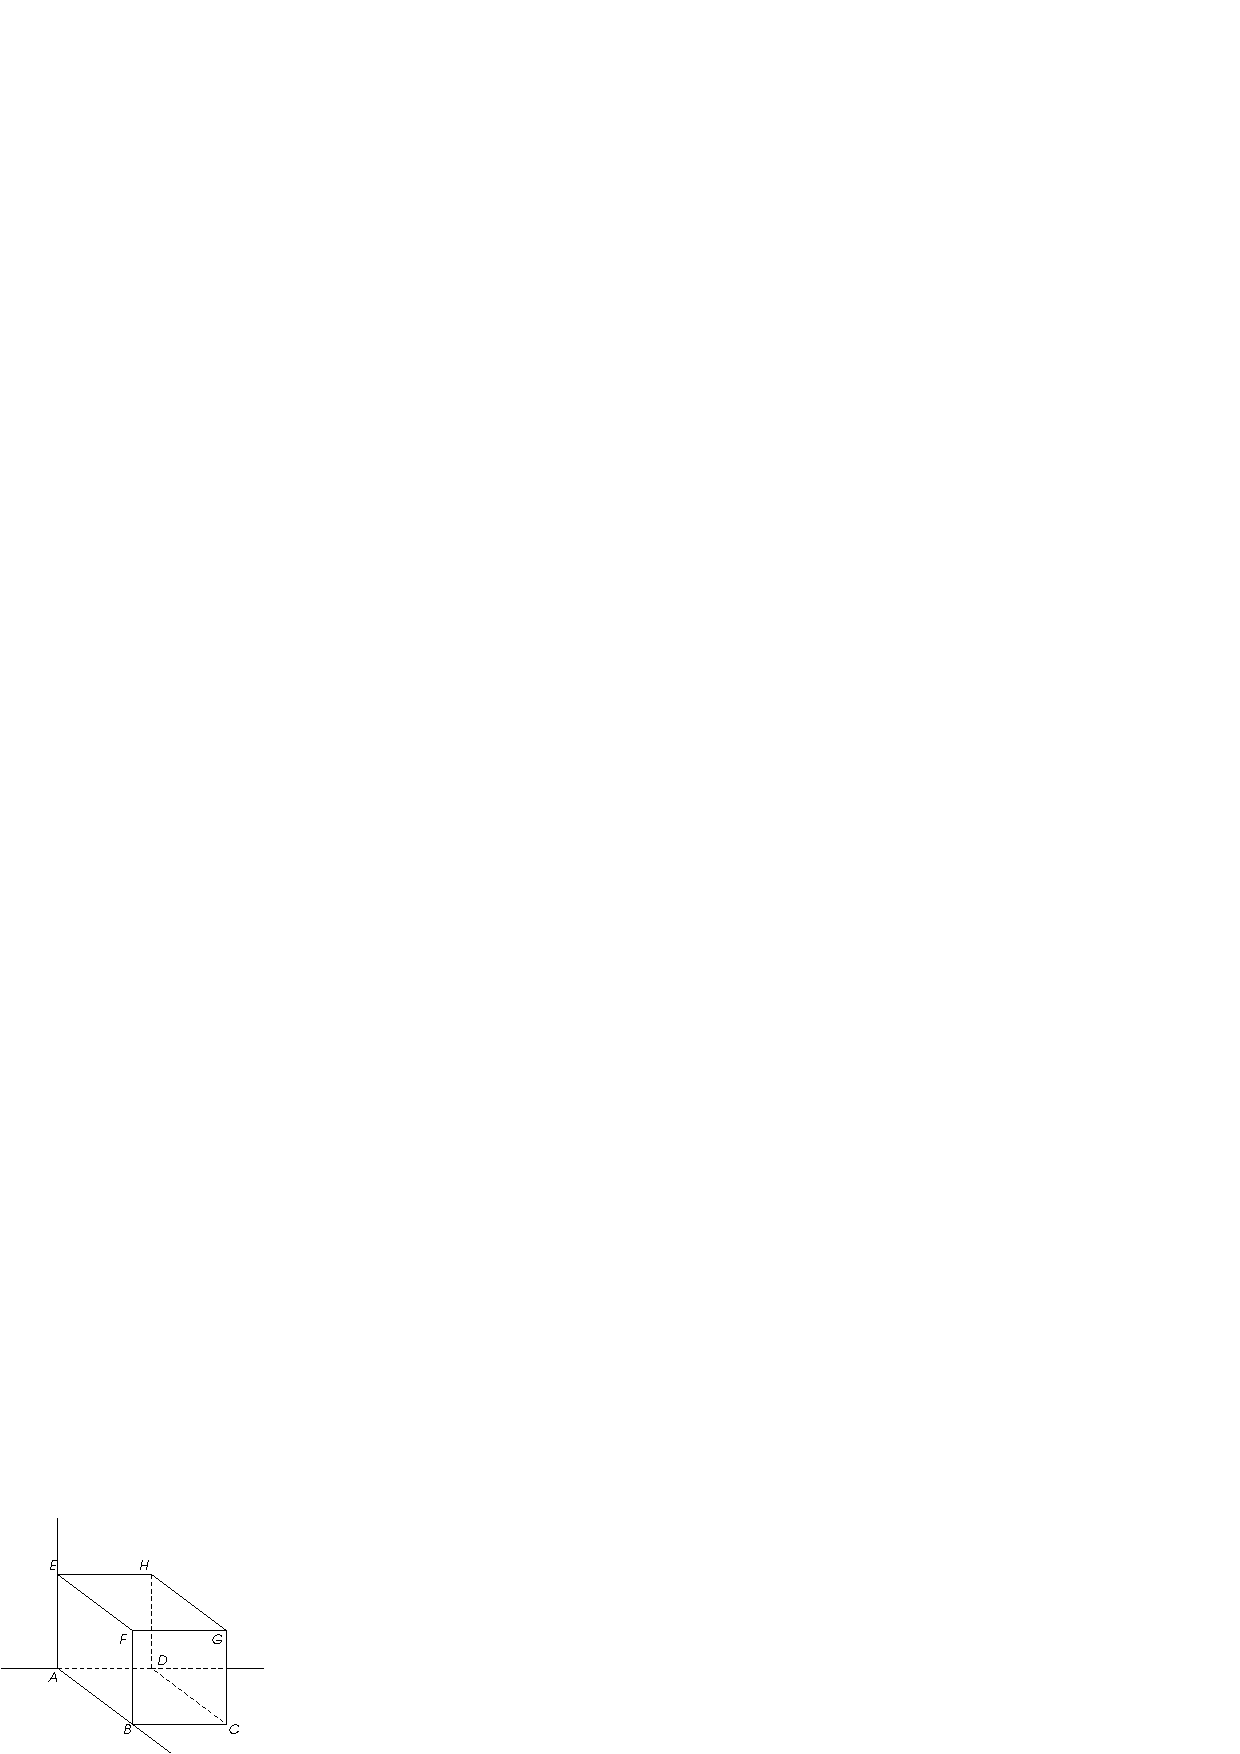
\includegraphics{05cube.pdf}
\end{center}
\problem \groupproblem  Let $\parppd ABCDEFGH$ be the cube with $A$ at the origin, 
$B(1,0,0)$, $D (0,1,0)$ and $E (0,0,1)$.

\subprob Find the coordinates of all the points $A$, $B$, $C$, $D$,
$E$, $F$, $G$, $H$.

\subprob Find the position vectors of the midpoints of the line
segments $AG$, $BH$, $CE$ and $DF$. Make a drawing of the cube with
these line segments.

\subprob Find the defining equation for the plane $BDE$. Do the same
for the plane $CFH$. Show that these planes are parallel.

\subprob Find the parametric equation for the line through $AG$.

\subprob Where do the planes $BDE$ and $CFH$ intersect the line $AG$?

\subprob Find the angle between the planes $BDE$ and $BGH$.

\subprob Find the angle between the planes $BDE$ and $BCH$. Draw these
planes.

\end{multicols}
\noproblemfont






